%! Author = Len Washington III
%! Date = 3/2/24

% Preamble
\documentclass[title={Chapter 8}]{fdsn201notes}

% Packages

% Document
\begin{document}

\maketitle{8}

\section{Regulating Metabolism}\label{sec:regulating-metabolism}
\begin{itemize}
	\item Vitamins and minerals do not contain Calories but assist in generating energy provided by macronutrients in the diet
\end{itemize}

\begin{figure}[H]
	\centering
	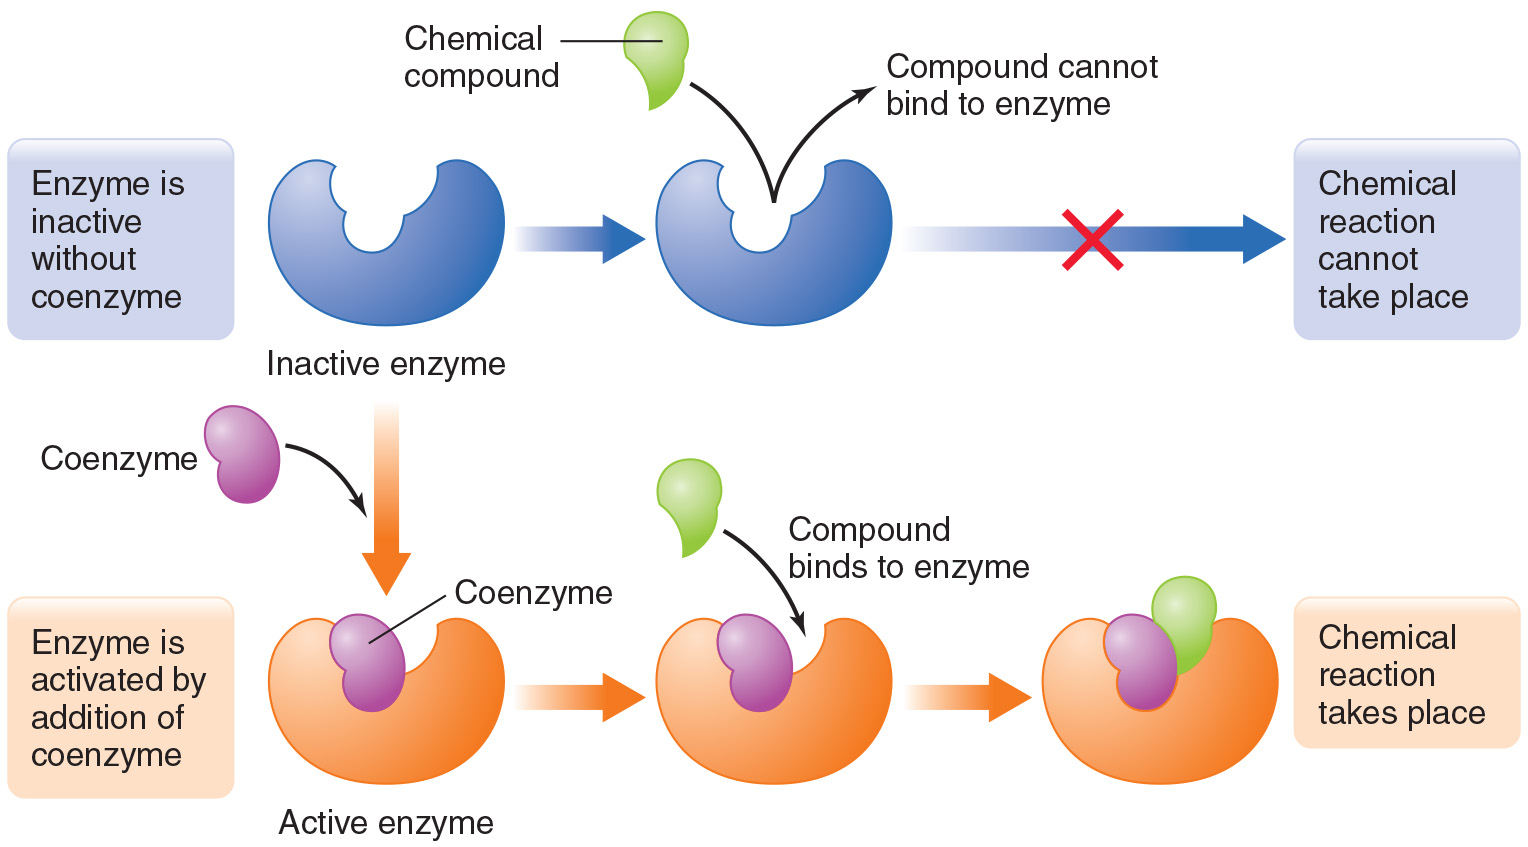
\includegraphics[width=\textwidth]{8_enzymes}
	\caption{Enzymes}
	\label{fig:enzymes}
\end{figure}

\begin{figure}[H]
	\centering
	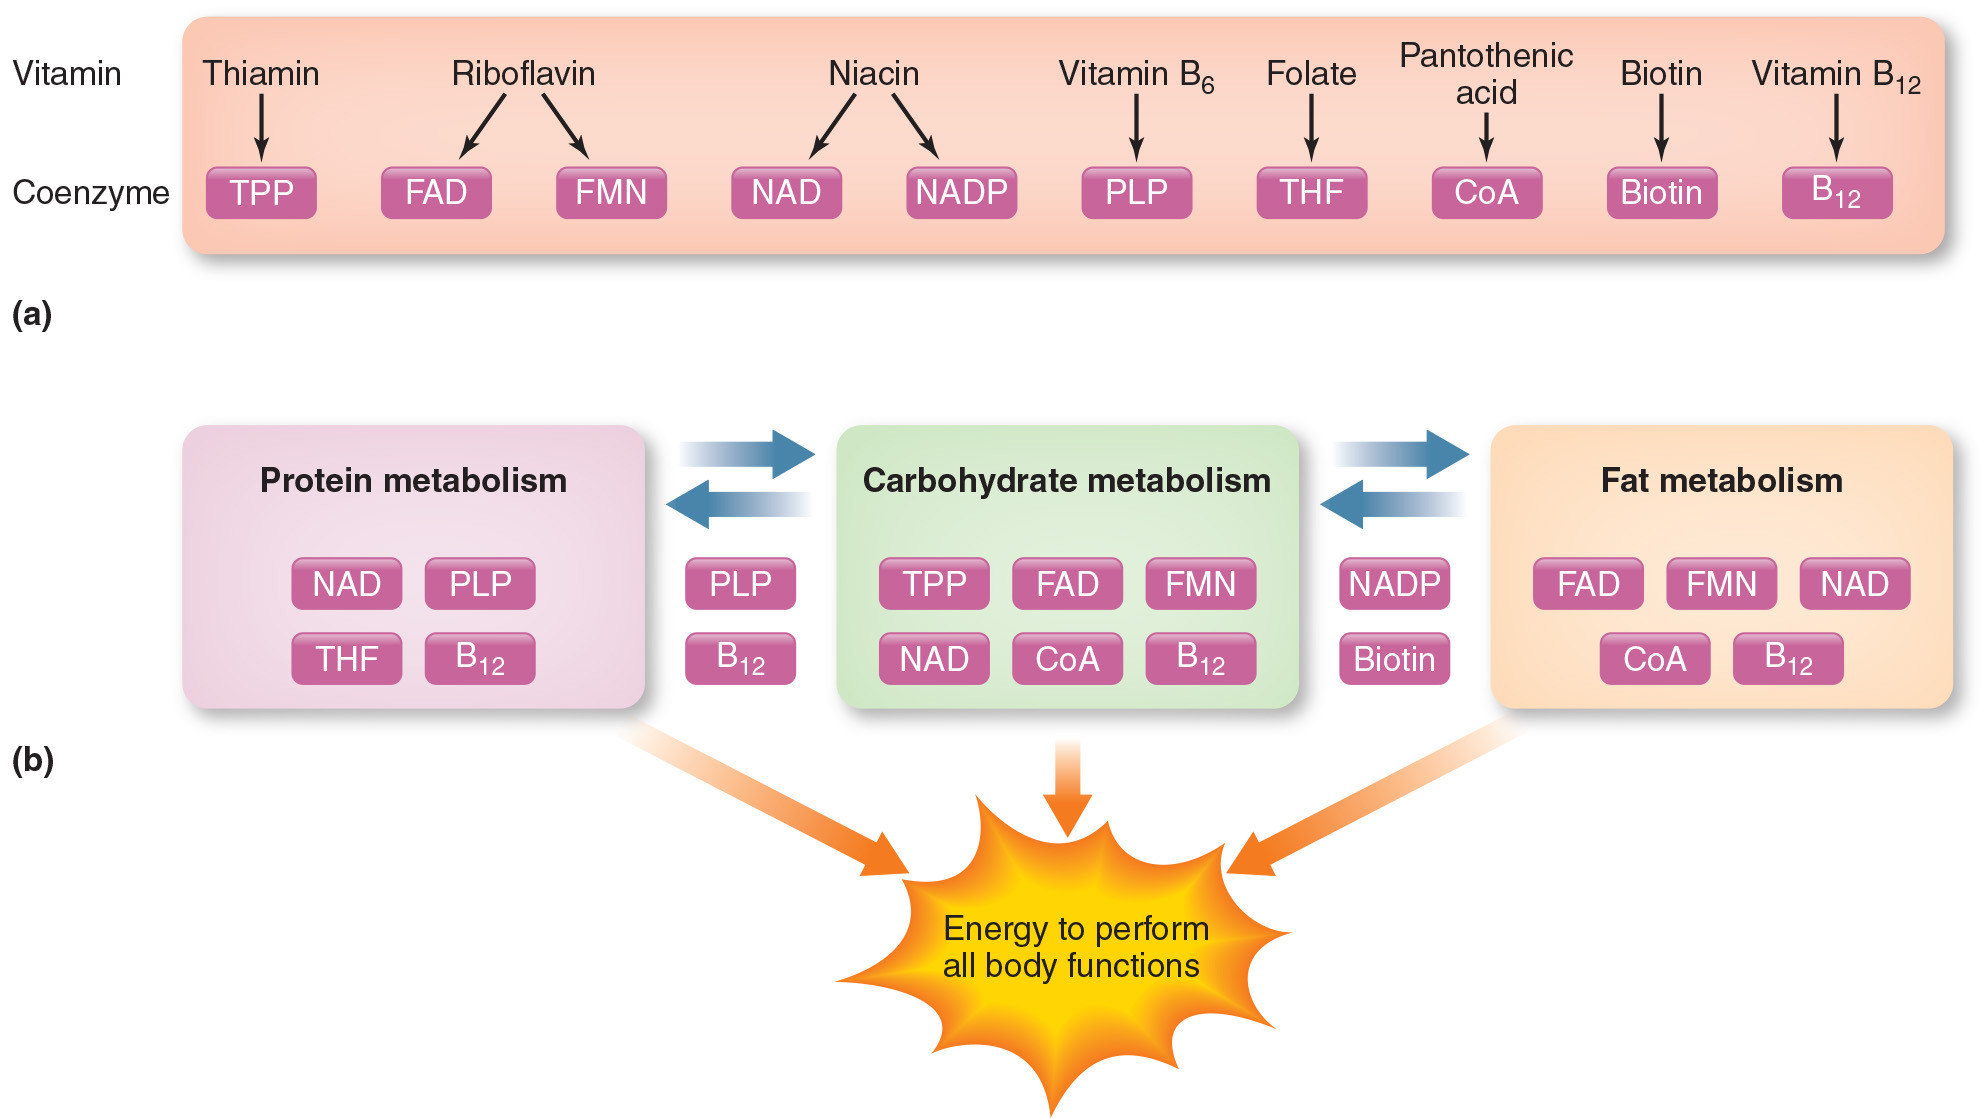
\includegraphics[width=\textwidth]{8_enzymes_continued}
	\caption{Enzymes}
	\label{fig:enzymes_continued}
\end{figure}

\begin{table}[H]
	\centering
	\begin{threeparttable}
		\caption{Nutrient and Energy Metabolism}
		\label{tab:nutrient-and-energy-metabolism}
		\rowcolors{2}{rowmedgreen}{rowlightgreen}
		\begin{tabular}{p{0.5\textwidth} p{0.5\textwidth}}
			\rowcolor{rowdarkgreen}\textbf{Nutrient} & \textbf{Recommended Intake}\\
			Thiamin (vitamin B1) & RDA for 19 years of age and older:

			Women = 1.1 mg/day

			Men = 1.2 mg/day\\

			Riboflavin (vitamin B2) & RDA for 19 years of age and older:

			Women 1.1 mg/day

			Men 1.3 mg/day\\
			Niacin (nicotinamide and nicotinic acid) & RDA for 19 years of age and older:

			Women 14 mg/day

			Men 16 mg/day \\
			Vitamin B6 (pyridoxine) & RDA for 19 to 50 years of age:

			1.3 mg/day

			RDA for 51 years of age and older:

			Women = 1.5 mg/day

			Men 1.7 mg/day\\
			Folate (folic acid) & RDA for 19 years of age and older

			400 $\mu$g/day\\
			Vitamin B12 (cobalamin) & RDA for 19 years of age and older:

			2.4 $\mu$g/day\\
			Pantothenic acid & Al for 19 years of age and older:

			5 mg/day\\
			Biotin & Al for 19 years of age and older:

			30 $\mu$g/day\\
			Choline & Al for 19 years of age and older:

			Women 425 mg/day

			Men 550 mg/day\\
			Iodine & RDA for 19 years of age and older:

			150 $\mu$g/day\\
			Chromium & RDA for 51 years of age and older:
			
			Women 20 $\mu$g/day
			
			Men 30 $\mu$g/day

			RDA for 19 to 50 years of age:

			Women 25 $\mu$g/day

			Men 35 $\mu$g/day\\
			Manganese & Al for 19 years of age and older:
			
			Women 1.8 mg/day
			
			Men = 2.3 mg/day\\
			Sulfur & No DRI.\\
			\rowcolor{rowdarkgreen} & \\
		\end{tabular}
		\begin{tablenotes}
			\small
			\item To see the full profile of all micronutrients, turn to the In Depth essay following Chapter 6, Vitamins and Minerals: Micronutrients with Macro Powers (pages 211--221).
		\end{tablenotes}
	\end{threeparttable}
\end{table}

\section{Thiamin ($\mbox{B}_{1}$)}\label{sec:thiamin}
\begin{itemize}
	\item Coenzyme that plays a critical role in carbohydrate metabolism
	\item Involved in the metabolism of branched chain amino acids
	\item Deficiency known as ``Beriberi''
	\item Sources include whole grains, pork, green vegetables, and okra.
\end{itemize}

\begin{figure}[H]
	\centering
	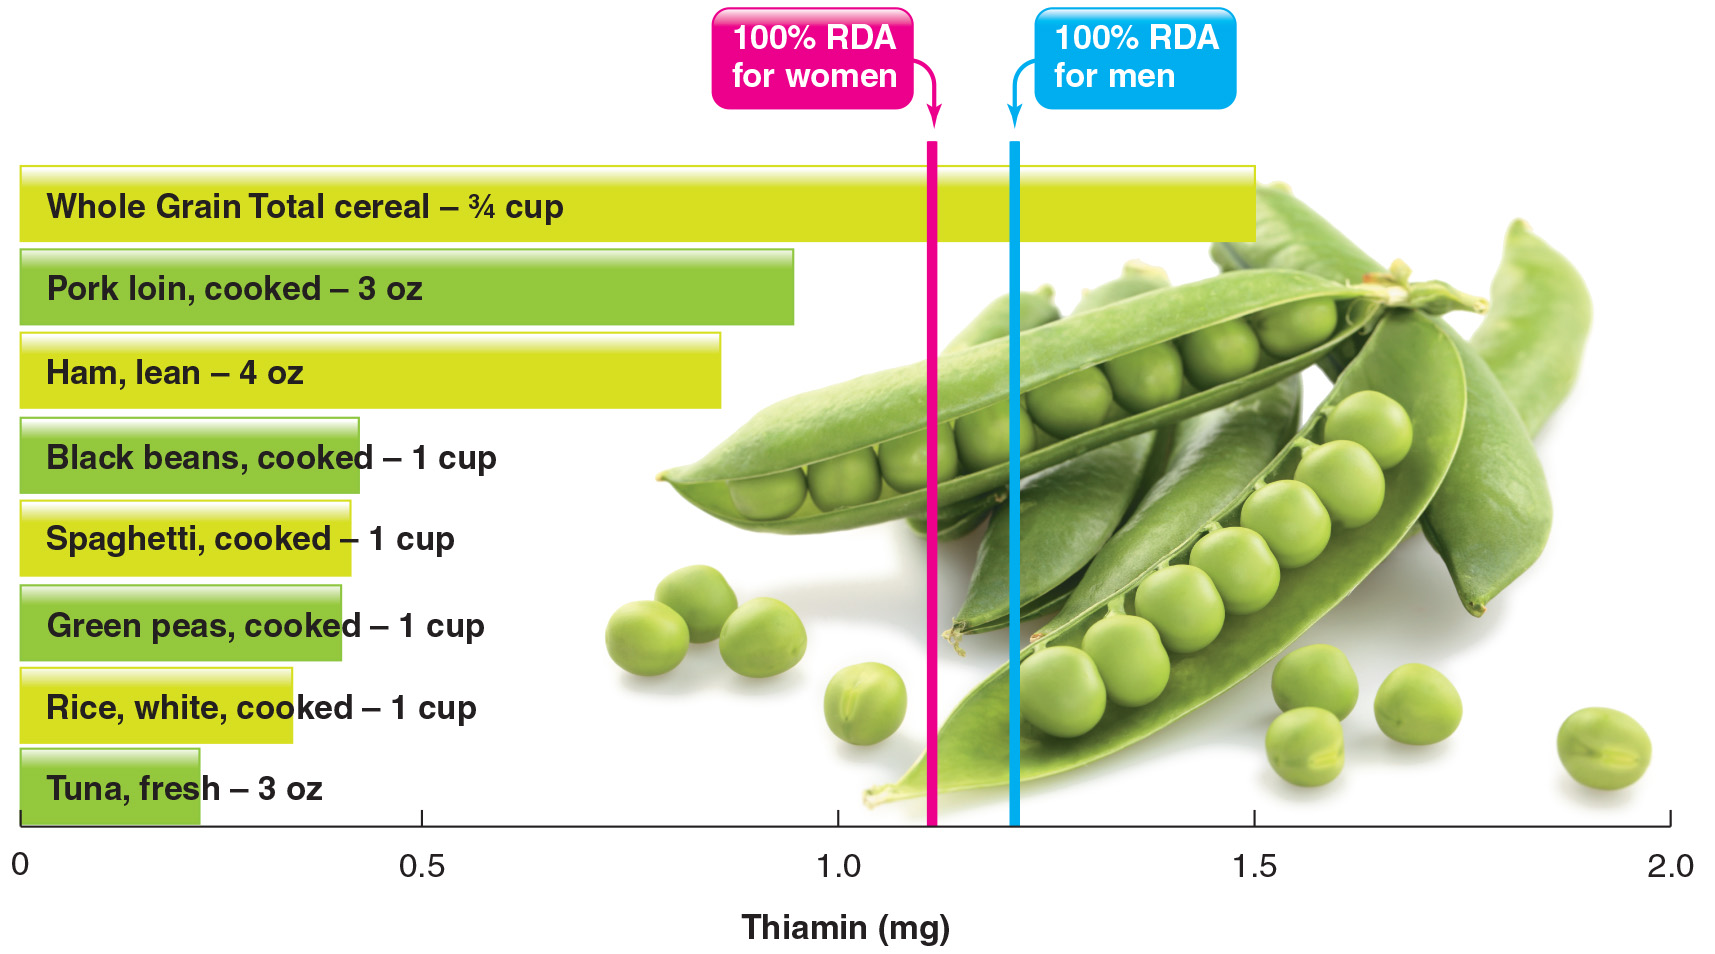
\includegraphics[width=\textwidth]{8_thiamin}
	\caption{Thiamin}
	\label{fig:thiamin}
\end{figure}

\section{Riboflavin ($\mbox{B}_{2}$)}\label{sec:riboflavin}
\begin{itemize}
	\item Coenzyme in the metabolism of carbohydrates and fats
	\item Deficiency is known as ariboflavinosis
	\item No known toxicity
	\item Sources include milk, fish, eggs, and poultry products
\end{itemize}

\begin{figure}[H]
	\centering
	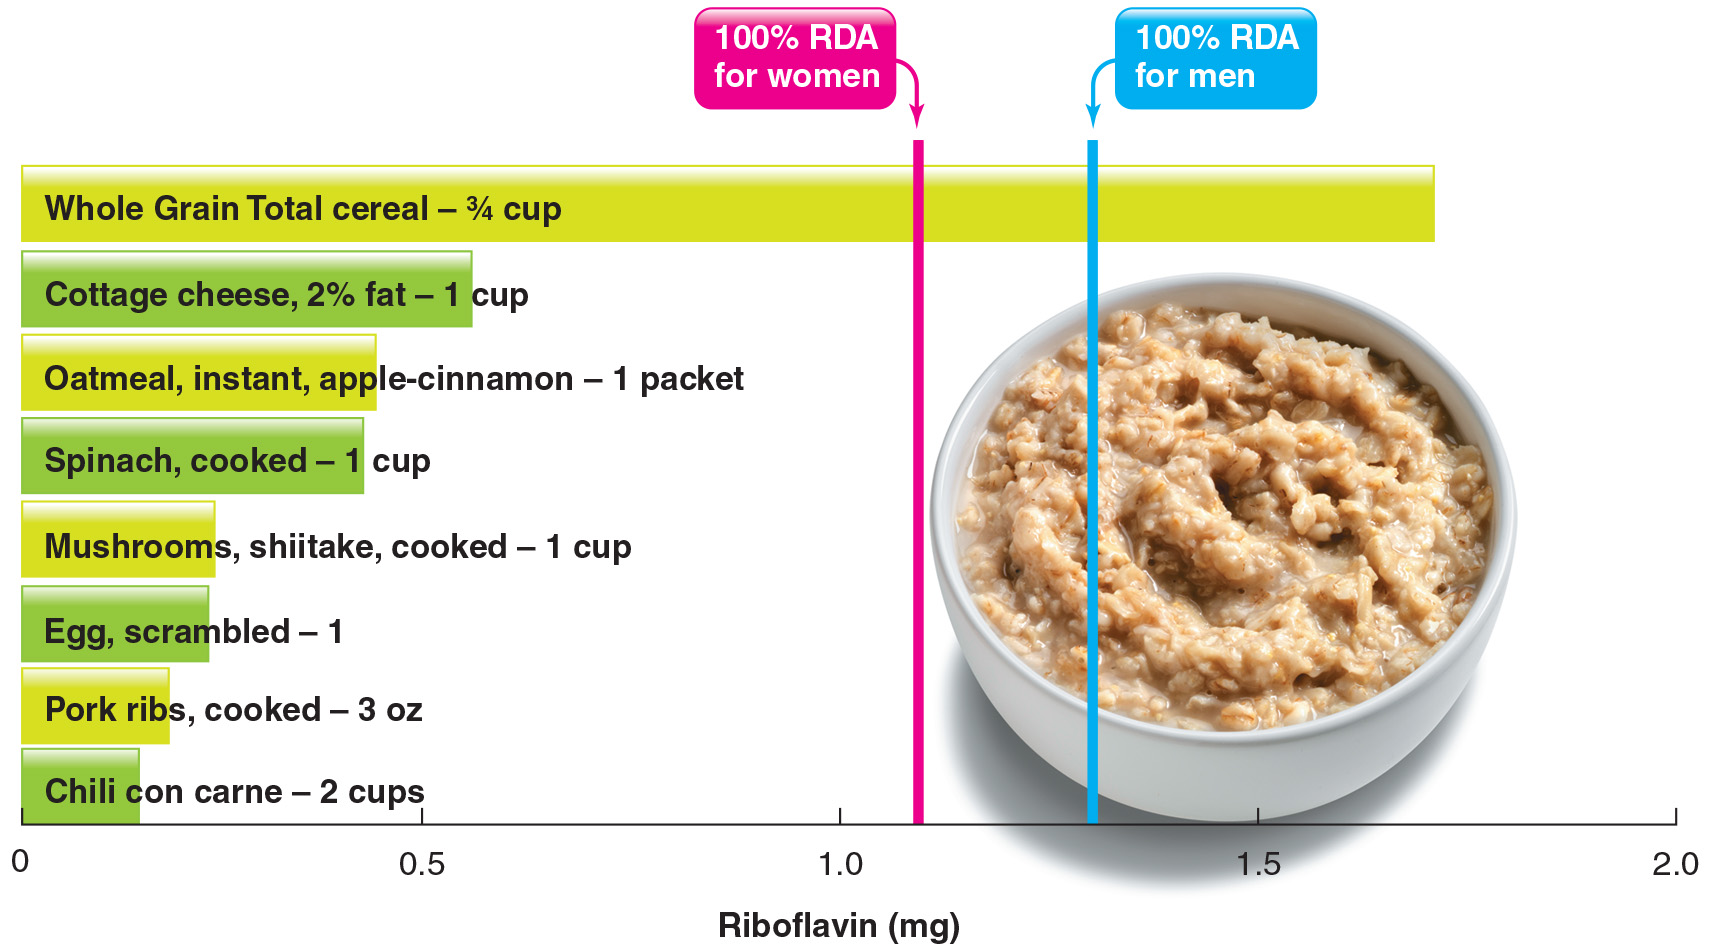
\includegraphics[width=\textwidth]{8_riboflavin}
	\caption{Riboflavin}
	\label{fig:riboflavin}
\end{figure}

\section{Niacin ($\mbox{B}_{3}$)}\label{sec:niacin}
\begin{itemize}
	\item Plays a role in the metabolism of carbohydrates and fatty acids
	\item Assists in DNA replication and cell differentiation
	\item Deficiency called pellagra
	\begin{itemize}
		\item Translated as ``angry skin''
		\begin{itemize}
			\item Dermatitis, diarrhea, dementia, and death
		\end{itemize}
	\end{itemize}
	\item Sources include meats, fish, and whole grains
\end{itemize}

\section{Pantothenic Acid ($\mbox{B}_{5}$)}\label{sec:Pantothenic Acid}
\begin{itemize}
	\item Component of all energy producing pathways
	\begin{itemize}
		\item Especially important for the breakdown and synthesis of fatty acids
	\end{itemize}
	\item Found in widespread food sources such as meats, eggs, potatoes, oats, tomatoes, whole grains, and yeast
\end{itemize}

\section{Pyrodoxine ($\mbox{B}_{6}$)}\label{sec:pyrodoxine}
involved in
\begin{itemize}
	\item Amino acid metabolism
	\item Neurotransmitter synthesis
	\item Carbohydrate metabolism
	\item Heme (hemoglobin) synthesis
	\item Immune function
	\item Reduction in cardiovascular disease
	\item Metabolism of other nutrients
\end{itemize}

\begin{figure}[H]
	\centering
	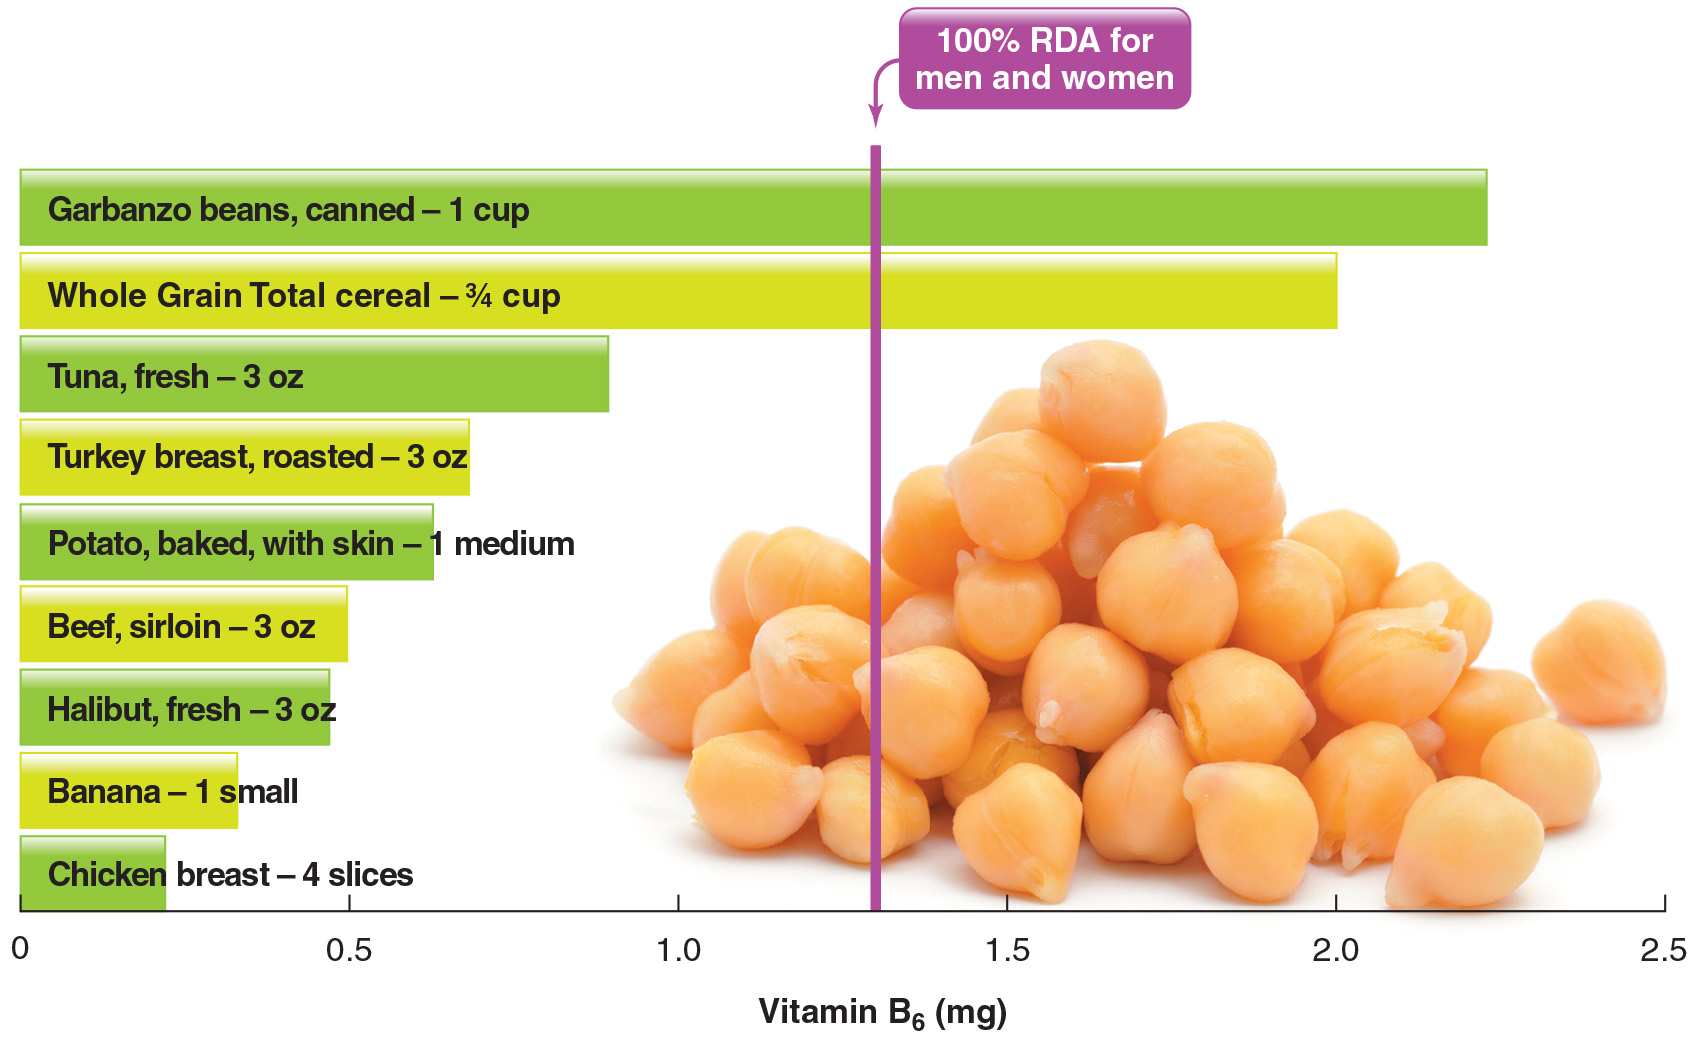
\includegraphics[width=\textwidth]{8_pyrodoxine}
	\caption{Pyrodoxine}
	\label{fig:pyrodoxine}
\end{figure}

\section{Folate ($\mbox{B}_{9}$)}\label{sec:folate}
\begin{itemize}
	\item Folate adds carbon units to other organic compounds
	\begin{itemize}
		\item Nucleotide synthesis
		\item Amino acid metabolism
		\item Red blood cell synthesis
		\item Critical role in spinal cord formation during pregnancy
	\end{itemize}
	\item Sources include leafy greens, fortified grain products, and ready to eat cereals
\end{itemize}

\begin{figure}[H]
	\centering
	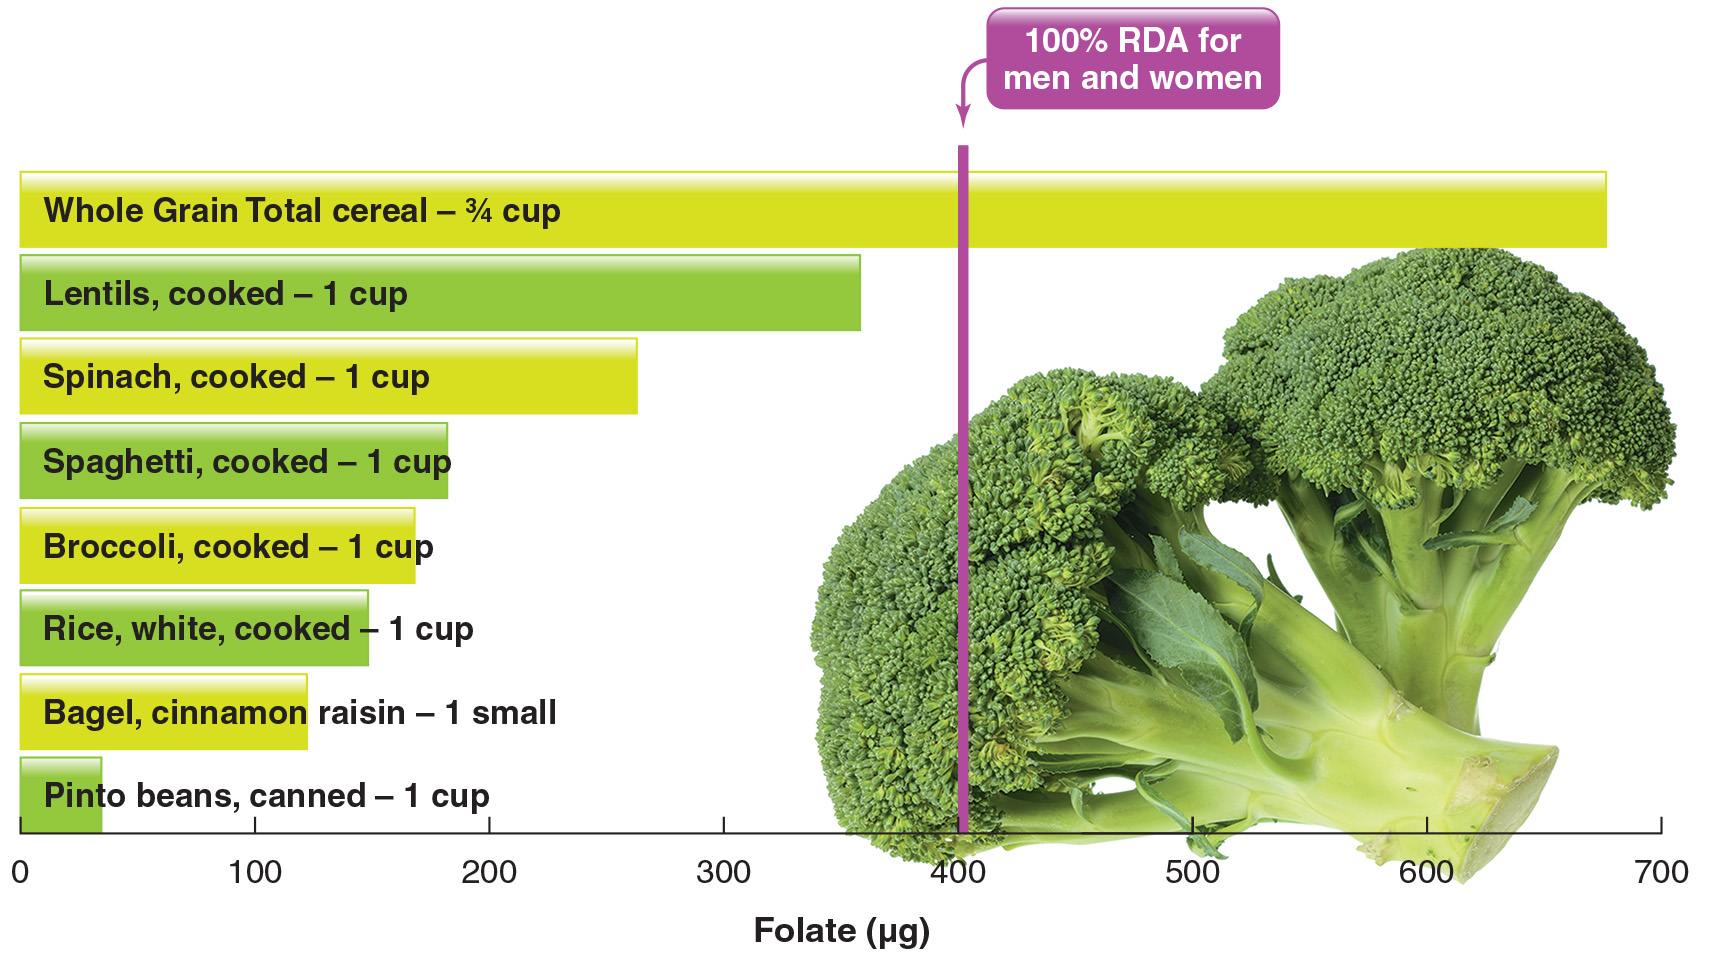
\includegraphics[width=\textwidth]{8_folate}
	\caption{Folate}
	\label{fig:folate}
\end{figure}

\section{Cobalamin ($\mbox{B}_{12}$)}\label{sec:b12}
\begin{itemize}
	\item Involved in metabolism of fatty acids
	\item Helps to maintain myelin sheath of nerves
	\item Helps to prevent the build up of homocysteine
	\item Sources include meats, dairy, eggs, fortified soy milk, and cereals
	\item No known toxicity
	\item Deficiency seen mainly in vegans
\end{itemize}

\begin{figure}[H]
	\centering
	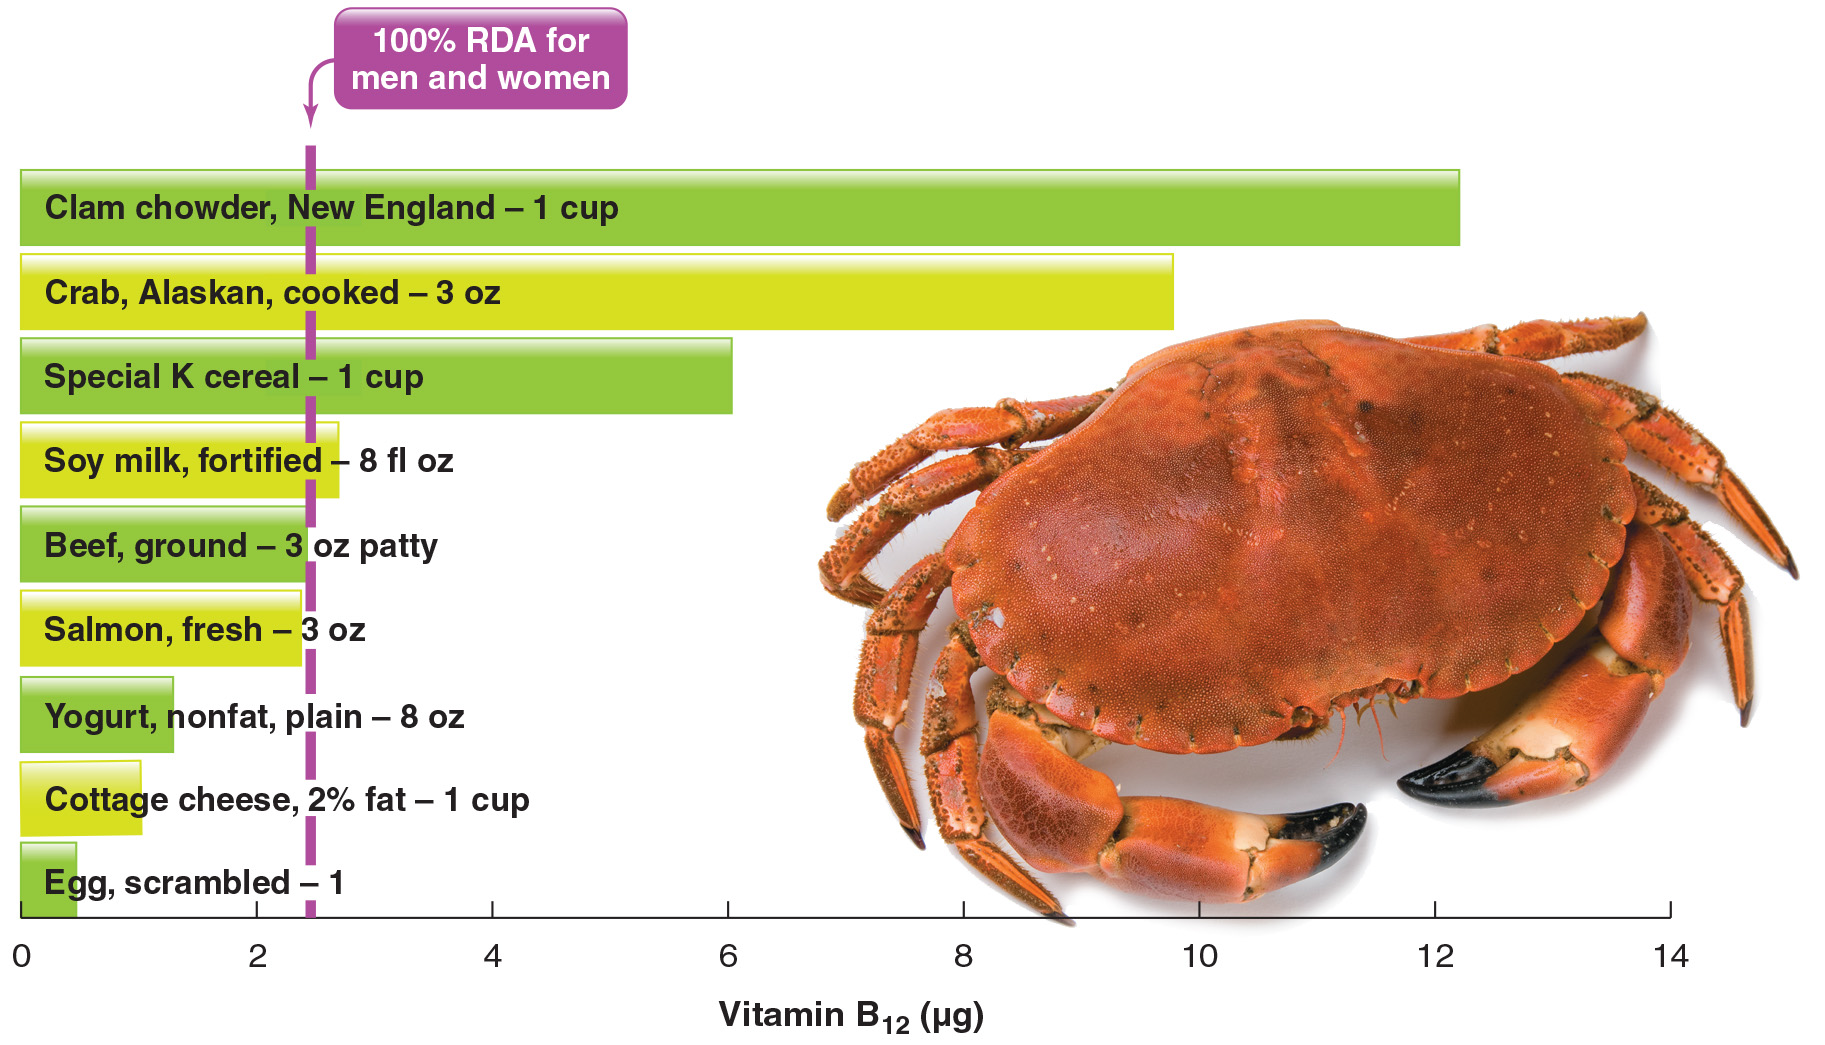
\includegraphics[width=\textwidth]{8_B12}
	\caption{$\mbox{B}_{12}$}
	\label{fig:B12}
\end{figure}

\section{Antioxidants}\label{sec:Antioxidants}
\begin{itemize}
	\item Micronutrients and phytochemicals that play a role in stabilizing free radicals include:
	\begin{itemize}
		\item Vitamins E, C, and A
		\item Minerals selenium, copper, iron, and manganese
	\end{itemize}
	\item Carotenoids such as beta-carotene also appear to have antioxidant properties
\end{itemize}

\section{Vitamin E}\label{sec:Vitamin E}
\begin{itemize}
	\item Vitamin E is a fat-soluble vitamin made of
	\begin{itemize}
		\item \definition{Tocotrienol}{biologically inactive form}
		\item \definition{Tocopherol}{biologically active form}
	\end{itemize}
	\item Functions of vitamin E
	\begin{itemize}
		\item Primary role is as an antioxidant
		\item Protects polyunsaturated fatty acids (PUFAs)
		\item Protects low-density lipoproteins (LDLs)
	\end{itemize}
	\item Recommended Dietary Allowance (RDA) is 15 mg alpha-tocopherol per day
	\begin{itemize}
		\item Tolerable upper limit (UL) is 1,000 mg per day
	\end{itemize}
	\item Sources of vitamin E
	\begin{itemize}
		\item Vegetable oils, nuts, seeds, wheat germ, soybeans
		\item Animal and dairy products are poor sources
	\end{itemize}
\end{itemize}

\begin{figure}[H]
	\centering
	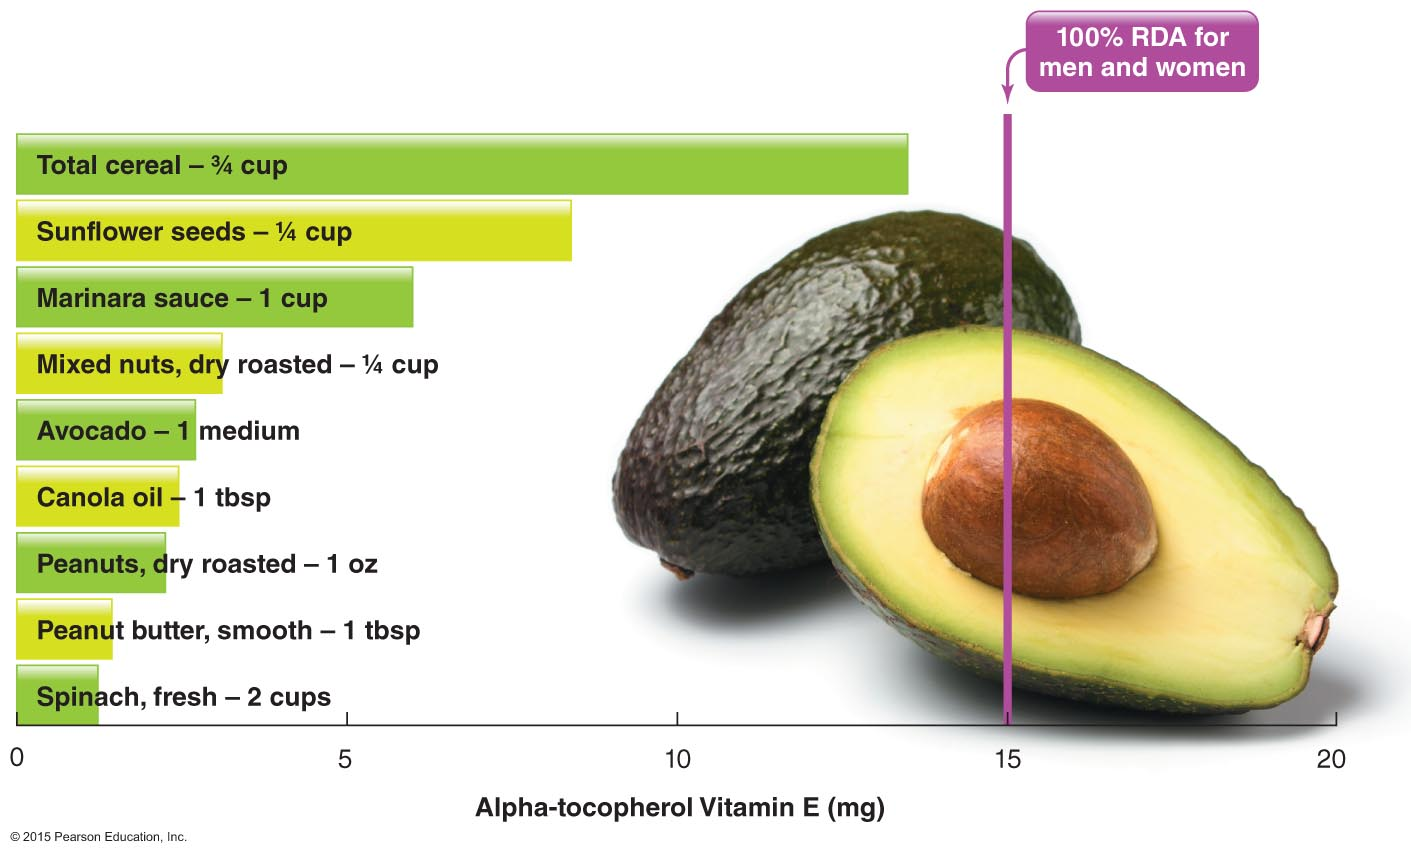
\includegraphics[width=\textwidth]{8_vitamin_e_common_sources}
	\caption{Common Food Sources of Vitamin E}
	\label{fig:common-food-sources-of-vitamin-e}
\end{figure}

\begin{itemize}
	\item What if you consume too much vitamin E?
	\begin{itemize}
		\item Some studies suggest possible links to vascular disease, diabetes, heart failure, and prostate cancer
		\item Side effects such as nausea, intestinal distress, and diarrhea have been reported
		\item Vitamin E can interfere with anticoagulant medications
		\item Tolerable upper limit (UL) is 1,000 mg per day
	\end{itemize}
	\item What if you don’t consume enough vitamin E?
	\begin{itemize}
		\item Vitamin E deficiencies are uncommon
		\item Can result in fragile red blood cells (erythrocyte hemolysis)
		\item Can cause loss of muscle coordination and reflexes
		\item Can impair immune function
	\end{itemize}
\end{itemize}

\section{Vitamin C}\label{sec:vitamin-c-8}
\begin{itemize}
	\item Vitamin C is a water-soluble vitamin that must be consumed in the human diet
	\item Functions of vitamin C
	\begin{itemize}
		\item Antioxidant
		\item Synthesis of collagen
		\item Prevents the disease scurvy
		\item Enhances the immune system
		\item Regenerates vitamin E after oxidation
		\item Enhances the absorption of iron
	\end{itemize}
	\item Recommended intake
	\begin{itemize}
		\item 90 mg/day for men; 75 mg/day for women
		\item Smokers need an extra 35 mg/day
		\item UL is 2,000 mg/day for adults
	\end{itemize}
	\item Sources of vitamin C
	\begin{itemize}
		\item Fresh fruits and vegetables
		\item Heat destroys vitamin C
		\item Cooking foods lowers their vitamin C content
	\end{itemize}
\end{itemize}

\begin{figure}[H]
	\centering
	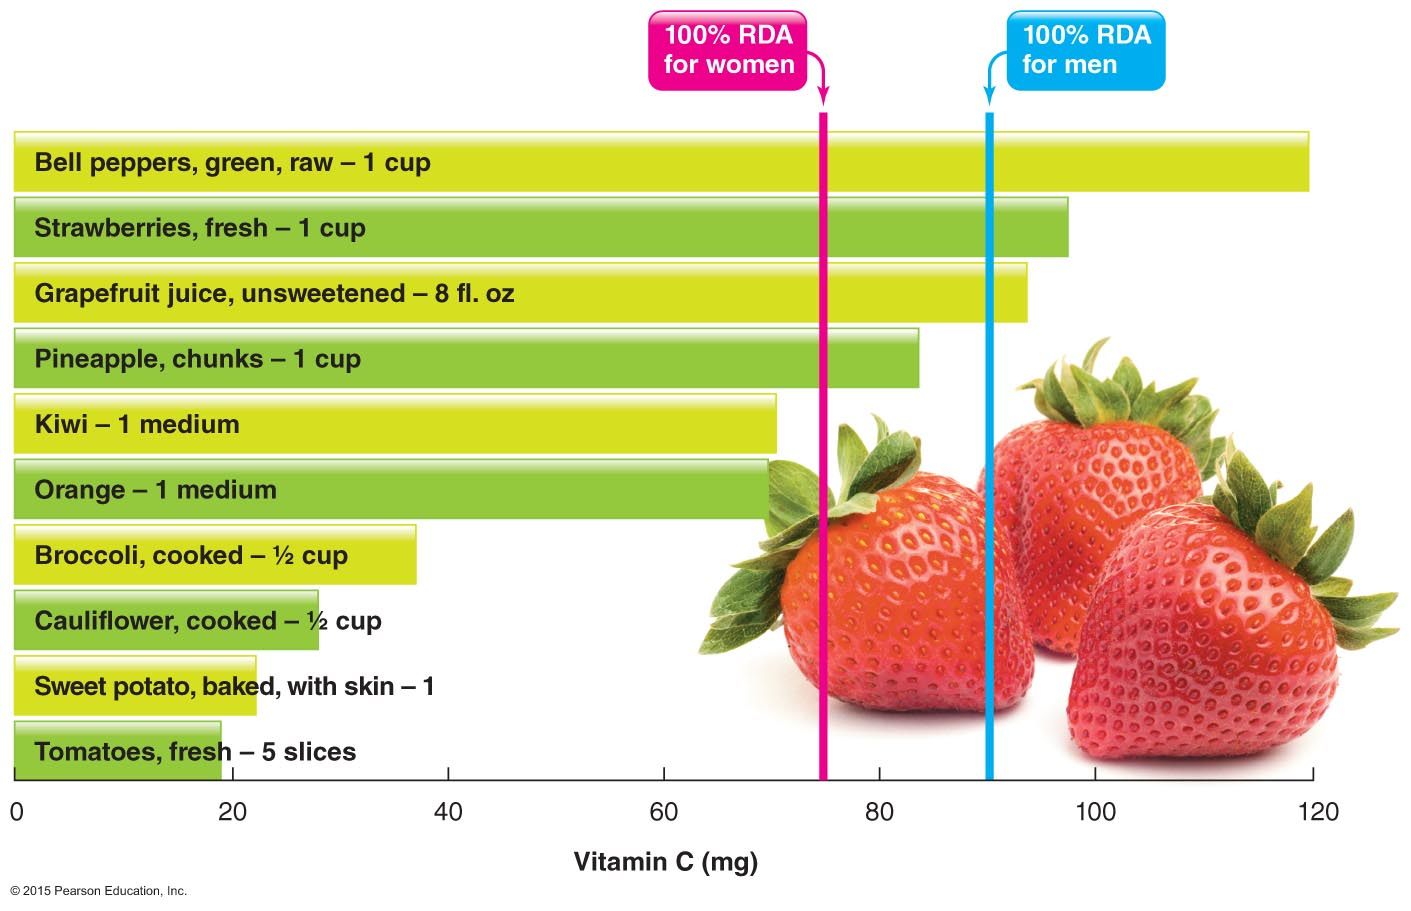
\includegraphics[width=\textwidth]{8_vitamin_c_common_sources}
	\caption{Common Food Sources of Vitamin C}
	\label{fig:common-food-sources-of-vitamin-c}
\end{figure}

\begin{itemize}
	\item What if you consume too much vitamin C?
	\begin{itemize}
		\item Megadoses (ten times or more of the recommended intake) of vitamin C can cause nausea, diarrhea, nosebleeds, and abdominal cramps
		\item Can cause iron toxicity in people with hemochromatosis
		\item Can lead to kidney stone formation in people with kidney disease
	\end{itemize}
	\item What if you don’t consume enough vitamin C?
	\begin{itemize}
		\item Scurvy is the most common vitamin C deficiency disease
		\item Bleeding gums, loose teeth, wounds that fail to heal, swollen ankles and wrists, bone pain and fractures, diarrhea, weakness, and depression
		\item Anemia can also result from vitamin C deficiency
	\end{itemize}
\end{itemize}

\begin{figure}[H]
	\centering
	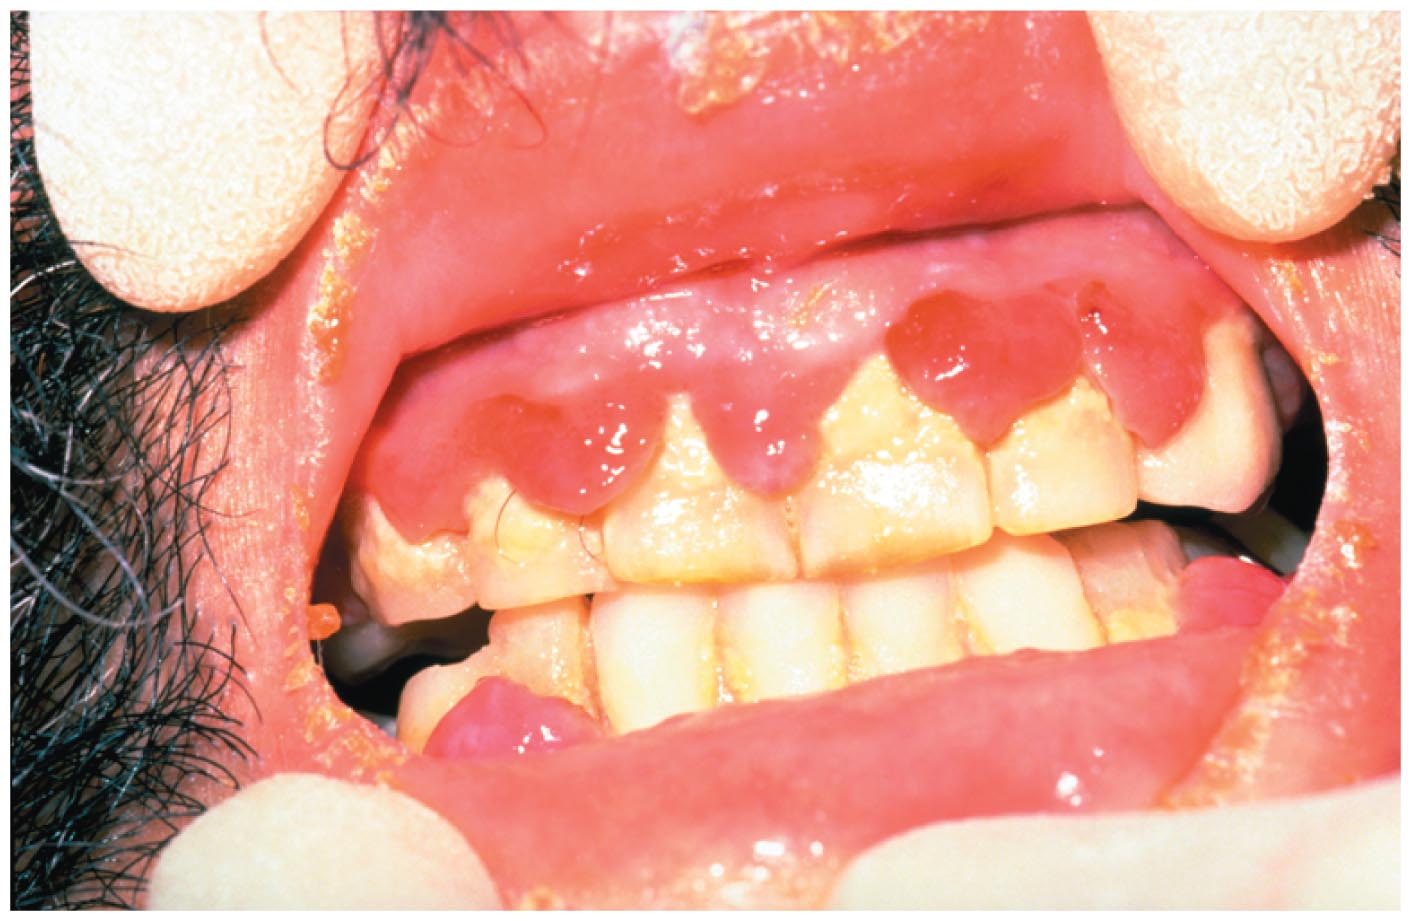
\includegraphics[width=\textwidth]{8_scurvy}
	\caption{Scurvy}
	\label{fig:scurvy}
\end{figure}

\section{Selenium}\label{sec:Selenium}
\begin{itemize}
	\item \definition{Selenium}{a trace mineral found in a few amino acids in the body}
	\item Functions of selenium
	\begin{itemize}
		\item Antioxidant--part of the glutathione peroxidase enzyme system
		\item Production of thyroxine, a thyroid hormone
	\end{itemize}
\end{itemize}

\begin{figure}[H]
	\centering
	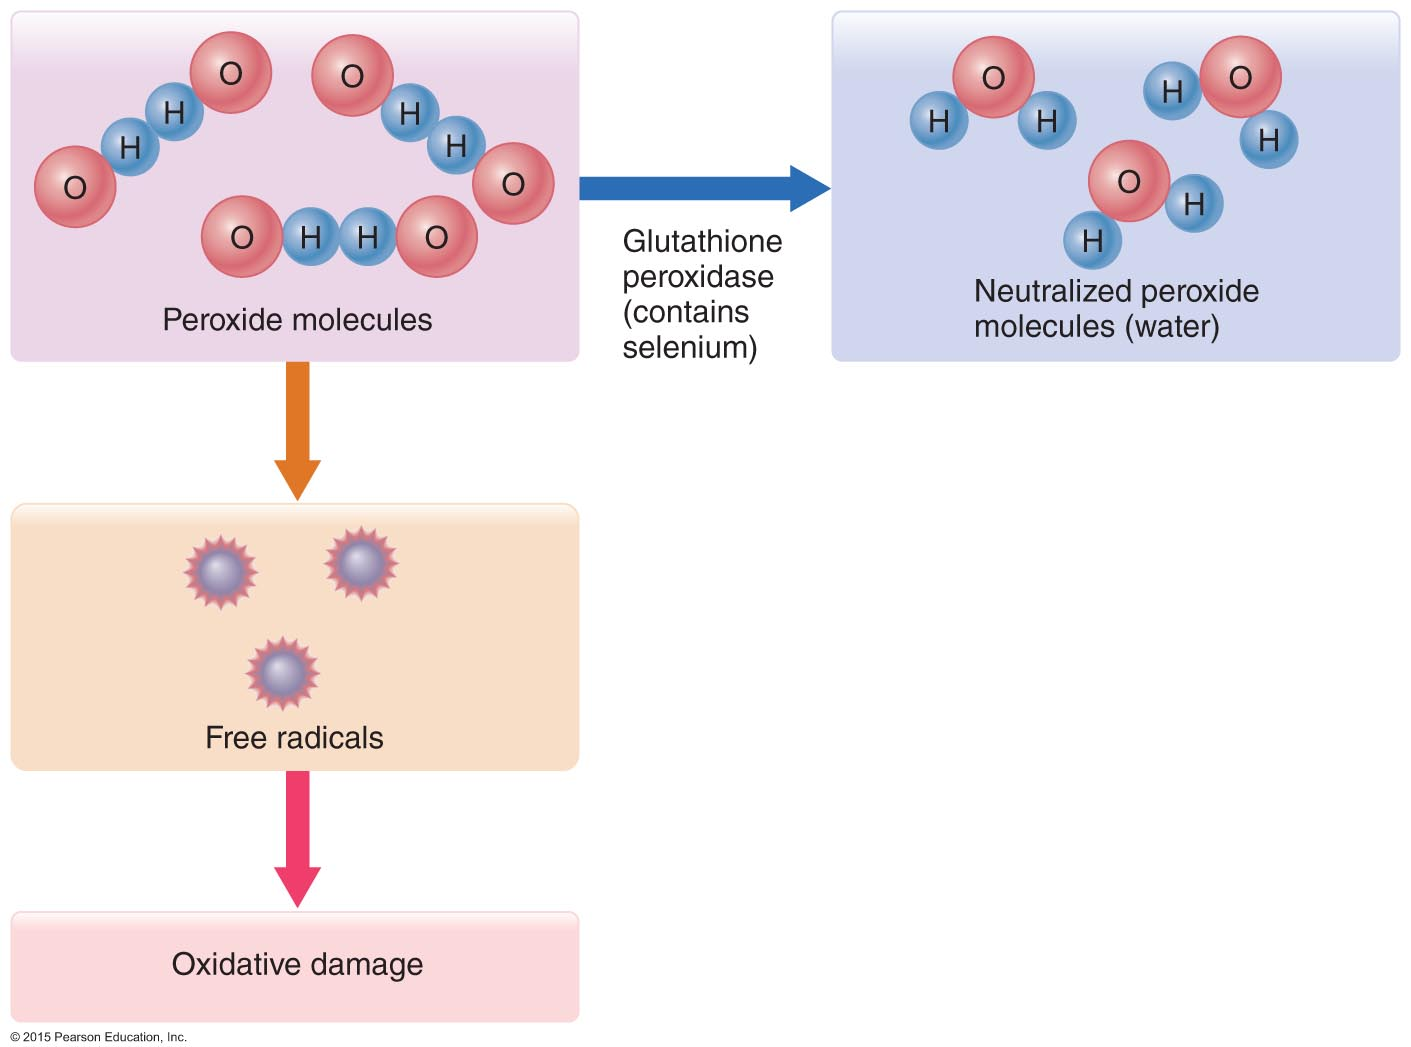
\includegraphics[width=\textwidth]{8_neutralizing_peroxide_molecules}
	\caption{Neutralizing Peroxide Molecules}
	\label{fig:neutralizing-peroxide-molecules}
\end{figure}

\begin{itemize}
	\item Recommended intake
	\begin{itemize}
		\item 55 µg/day for men and women
		\item UL is 400 µg/day
	\end{itemize}
	\item Sources of selenium
	\begin{itemize}
		\item Rich sources include organ meats, pork, seafood, fish, and nuts
	\end{itemize}
\end{itemize}

\begin{figure}[H]
	\centering
	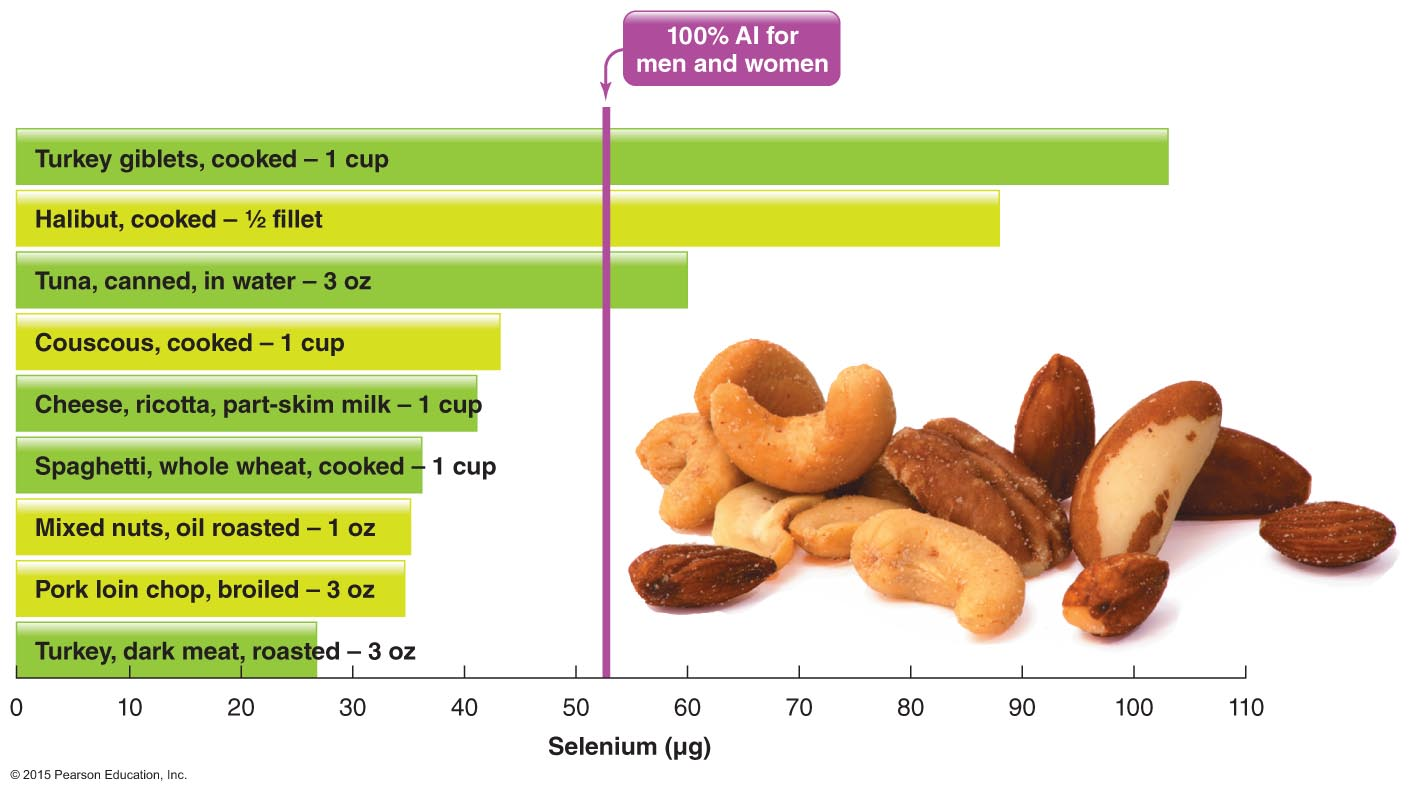
\includegraphics[width=\textwidth]{8_selenium_common_sources}
	\caption{Common Food Sources of Selenium}
	\label{fig:common-food-sources-of-selenium}
\end{figure}

\begin{itemize}
	\item What if you consume too much selenium?
	\begin{itemize}
		\item Selenium toxicity (brittle hair, nails, skin rashes) can result from supplements
	\end{itemize}
	\item What if you don’t consume enough selenium?
	\begin{itemize}
		\item \definition{Keshan disease}{a form of heart disease}
		\item \definition{Kashin-Beck disease}{a type of arthritis}
	\end{itemize}
\end{itemize}

\begin{figure}[H]
	\centering
	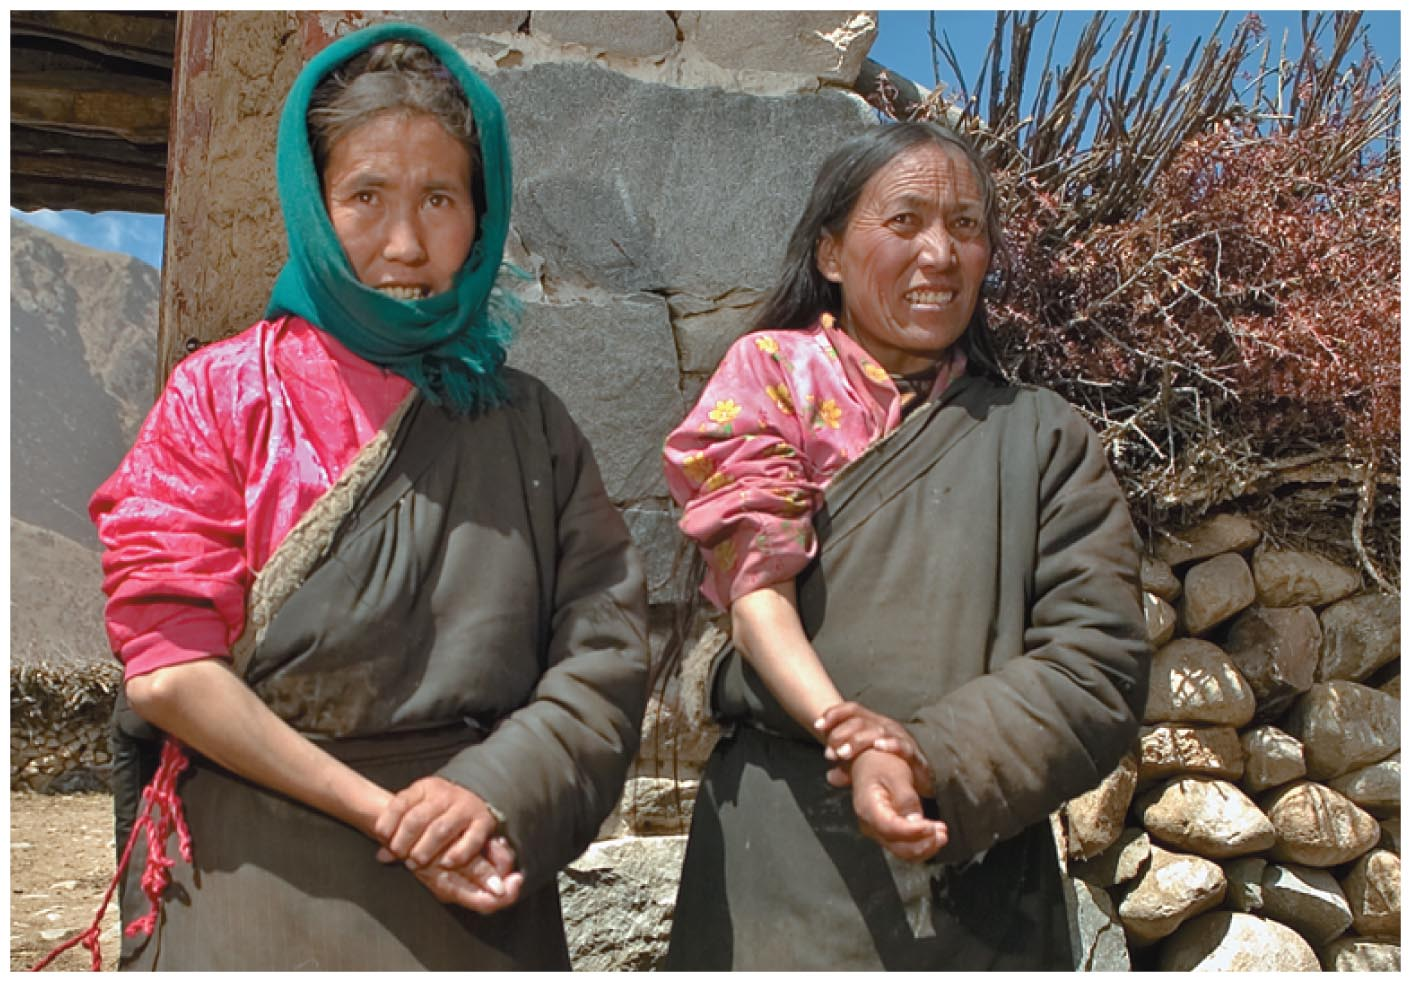
\includegraphics[width=\textwidth]{8_kashin_beck_disease}
	\caption{Kashin-Beck Disease}
	\label{fig:kashin-beck-disease}
\end{figure}


\section{Copper, Iron, Zinc, and Manganese}\label{sec:copper-iron-zinc-and-manganese}
\definition{Cofactor}{a compound needed for proper functioning of an enzyme}
\begin{itemize}
	\item Copper, zinc, and manganese are cofactors for the superoxide dismutase antioxidant enzyme system
	\item Copper, iron, and zinc help us maintain the health of our blood
	\item Manganese is an important cofactor in carbohydrate (CHO) metabolism
\end{itemize}

\section{Beta-Carotene}\label{sec:beta-carotene}
\begin{itemize}
	\item In the class of chemicals called carotenoids
	\item A provitamin: inactive precursors that must be converted to the active form of a vitamin in the body
	\item The precursor of retinol, an active form vitamin A
	\item Functions of beta-carotene
	\begin{itemize}
		\item A relatively weak antioxidant
		\item Effective against oxidation in cell membranes and LDLs
	\end{itemize}
	\item Carotenoids in general are known to
	\begin{itemize}
		\item Enhance the immune system
		\item Protect skin from damage by UV light
		\item Protect eyes from damage
	\end{itemize}
	\item Recommended intake
	\begin{itemize}
		\item Beta-carotene is not considered an essential nutrient
		\item No RDA has been established
	\end{itemize}
	\item Sources of beta-carotene
	\begin{itemize}
		\item Fruits and vegetables that are red, orange, yellow, and deep green
		\item Carotenoids are better absorbed from cooked foods
	\end{itemize}
\end{itemize}

\begin{figure}[H]
	\centering
	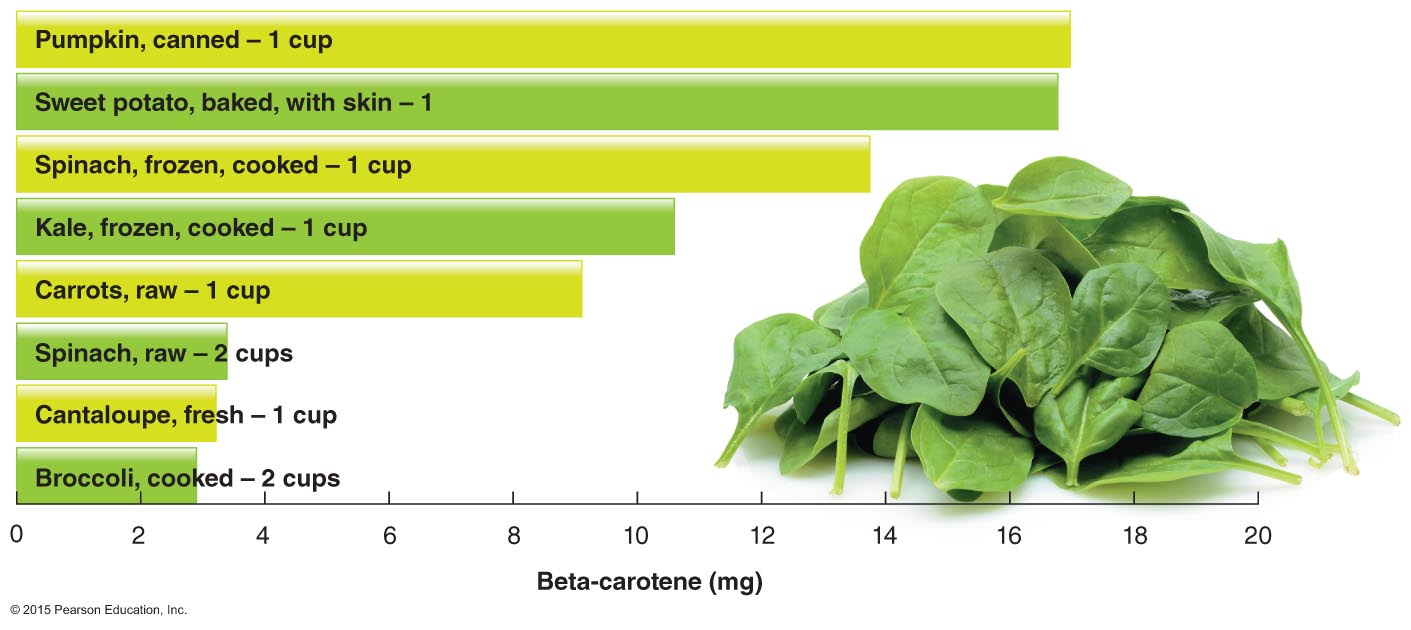
\includegraphics[width=\textwidth]{8_beta_carotene_common_sources}
	\caption{Common Food Sources of Beta-Carotene}
	\label{fig:common-food-sources-of-beta}
\end{figure}

\begin{itemize}
	\item What if you consume too much beta-carotene?
	\begin{itemize}
		\item Large quantities do not appear to be toxic
		\item Skin may turn yellow or orange at high intakes; harmless and reversible
	\end{itemize}
	\item What if you don’t consume enough beta-carotene?
	\begin{itemize}
		\item There are no known deficiency symptoms
	\end{itemize}
\end{itemize}

\section{Vitamin A}\label{sec:Vitamin A}
\begin{itemize}
	\item Vitamin A is a fat-soluble vitamin
	\begin{itemize}
		\item Excess vitamin A is stored in the liver, adipose tissue, kidneys, and lungs
		\item There are three active forms of vitamin A
		\begin{itemize}
			\item Retinol
			\item Retinal
			\item Retinoic acid
		\end{itemize}
	\end{itemize}
\end{itemize}

\begin{figure}[H]
	\centering
	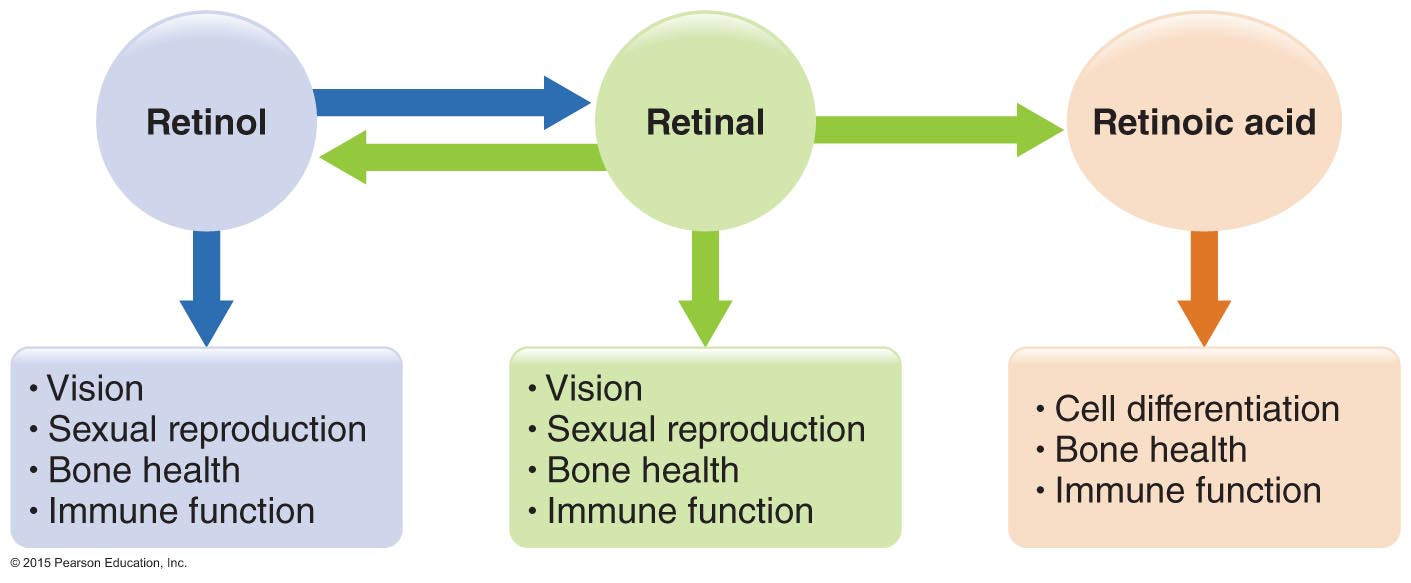
\includegraphics[width=\textwidth]{8_vitamin_a_active_forms}
	\caption{The Three Active Forms of Vitamin A}
	\label{fig:vitamin-a-active-forms}
\end{figure}

\begin{itemize}
	\item Functions of vitamin A
	\begin{itemize}
		\item Contributes to cell differentiation
		\item Contributes to reproduction and bone growth
		\item May act as an antioxidant
		\item Essential to sight
	\end{itemize}
\end{itemize}

\begin{figure}[H]
	\centering
	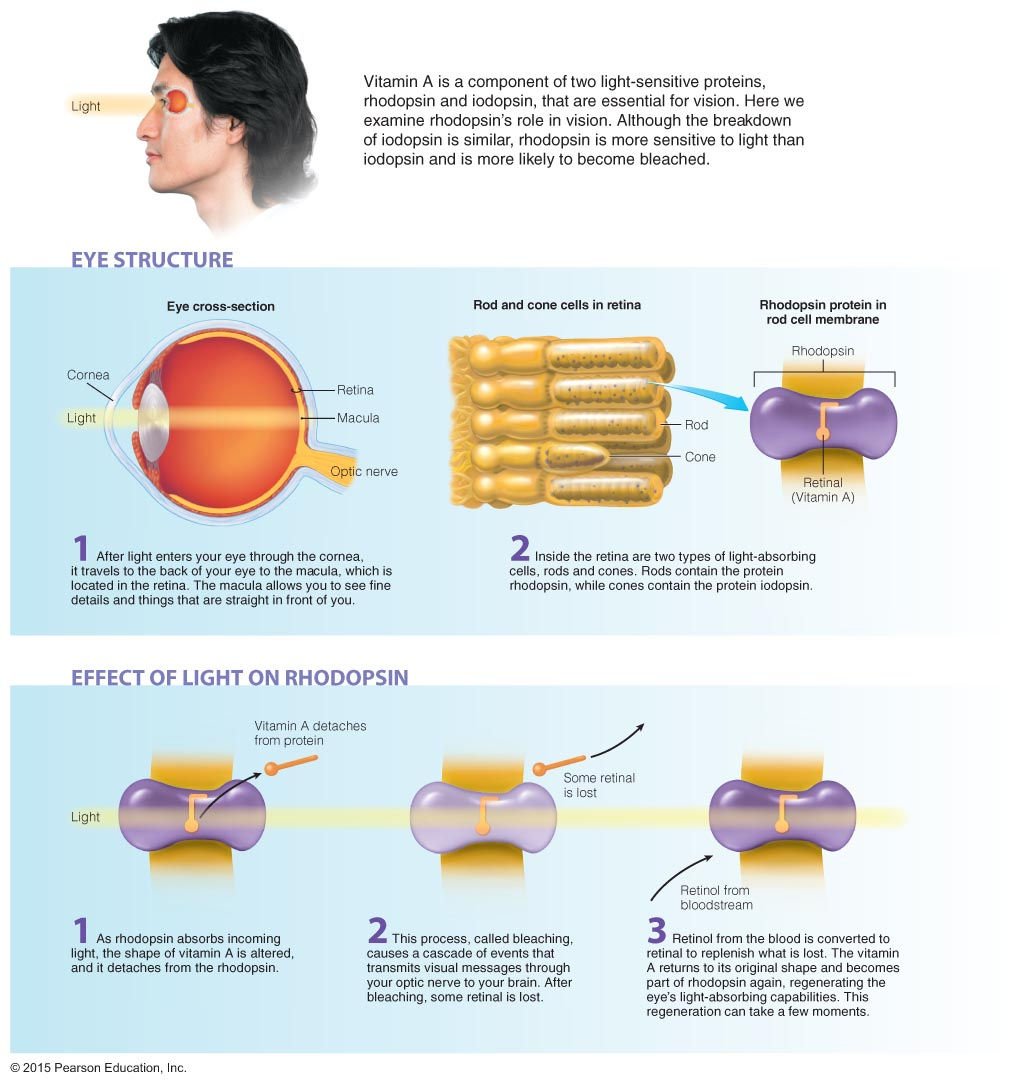
\includegraphics[width=\textwidth]{8_vitamin_a_essential_to_sight}
	\caption{Vitamin A Is Essential to Sight}
	\label{fig:vitamin-a-is-essential-to-sight}
\end{figure}

\begin{figure}[H]
	\centering
	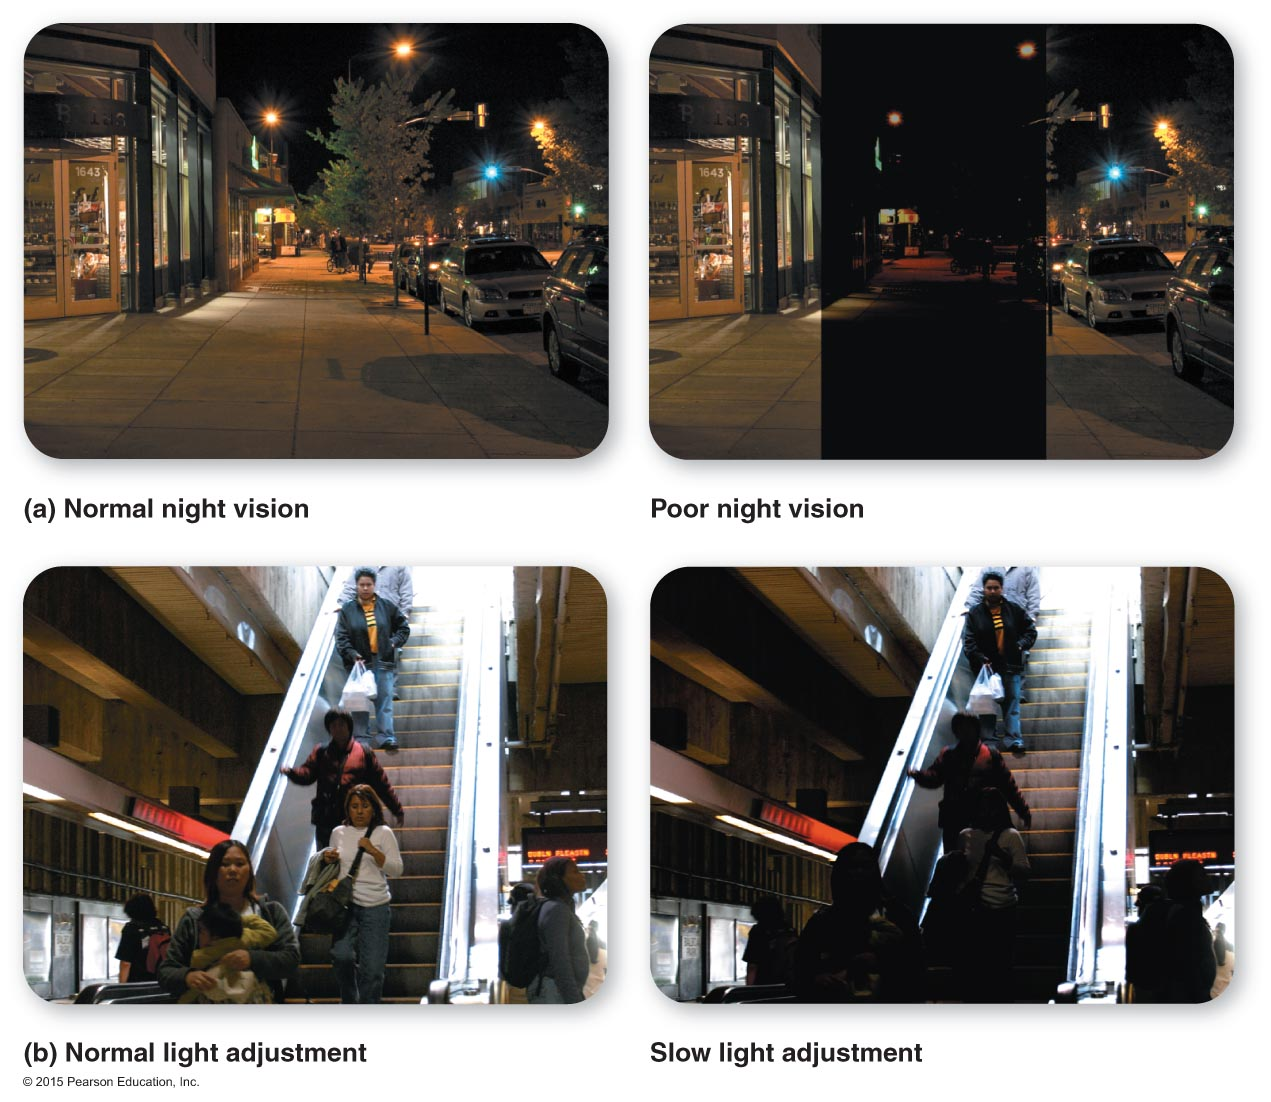
\includegraphics[width=\textwidth]{8_vitamin_a_essential_to_sight-2}
	\caption{Vitamin A Is Essential to Sight}
	\label{fig:vitamin-a-is-essential-to-sight-cont}
\end{figure}

\begin{itemize}
	\item Recommended intake
	\begin{itemize}
		\item RDA is 900 µg/day for men, 700 µg/day for women
	\end{itemize}
	\item Sources of vitamin A
	\begin{itemize}
		\item Animal sources: liver, eggs
		\item Plant sources such as the provitamin carotenoids (dark-green, orange, and deep-yellow fruits and vegetables)
	\end{itemize}
\end{itemize}

\begin{figure}[H]
	\centering
	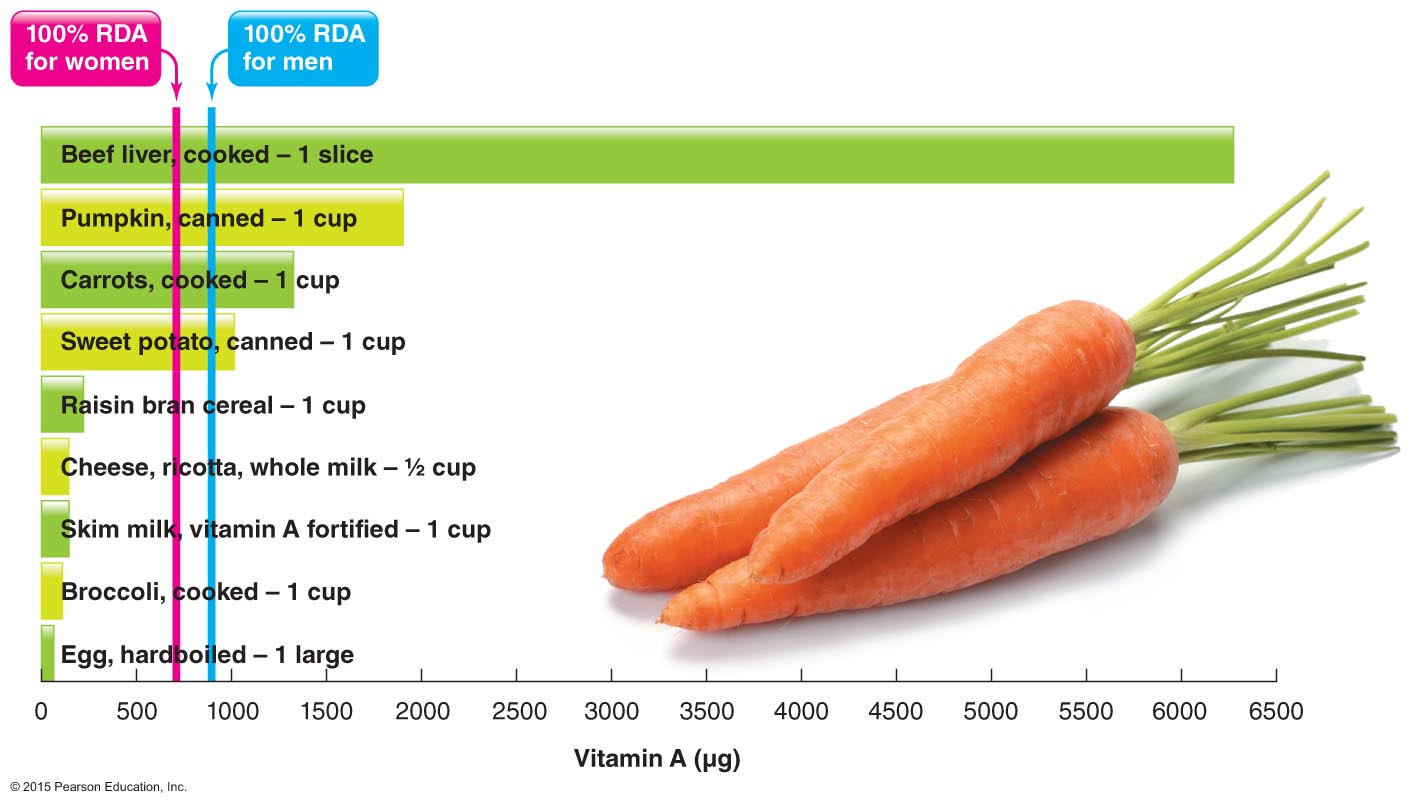
\includegraphics[width=\textwidth]{8_vitamin_a_common_sources}
	\caption{Common Food Sources of Vitamin A}
	\label{fig:common-food-sources-of-vitamin-a}
\end{figure}

\begin{itemize}
	\item What if you consume too much vitamin A?
	\begin{itemize}
		\item Vitamin A is highly toxic, especially from supplements
		\item Birth defects and permanent damage to the liver and eyes can result
	\end{itemize}
	\item What if you don’t consume enough vitamin A?
	\begin{itemize}
		\item Night blindness is the most common disease of vitamin A deficiency
		\item Irreversible blindness (xerophthalmia)
	\end{itemize}
\end{itemize}

\section{In Depth: Cancer}\label{sec:in-depth:-cancer}
\begin{itemize}
	\item \definition{Cancer}{a group of related diseases characterized by cells growing out of control}
	\begin{itemize}
		\item Composed of three steps
		\begin{itemize}
			\item \definition{Initiation}{a cell’s DNA is mutated}
			\item \definition{Promotion}{altered cell repeatedly divides}
			\item \definition{Progression}{cells grow out of control}
		\end{itemize}
	\end{itemize}
\end{itemize}

\begin{figure}[H]
	\centering
	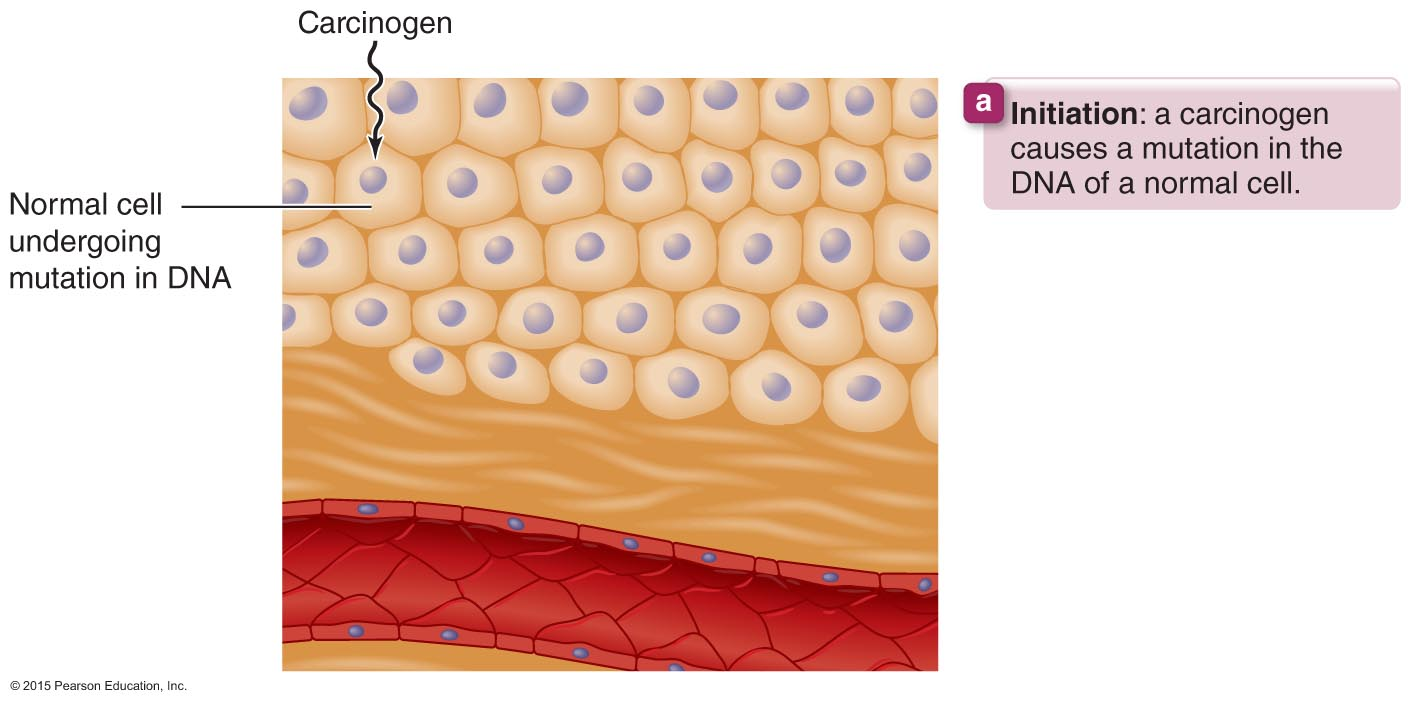
\includegraphics[width=\textwidth]{8_cancer_initiation}
	\caption{Cancer Initiation}
	\label{fig:cancer-initiation}
\end{figure}


\begin{figure}[H]
	\centering
	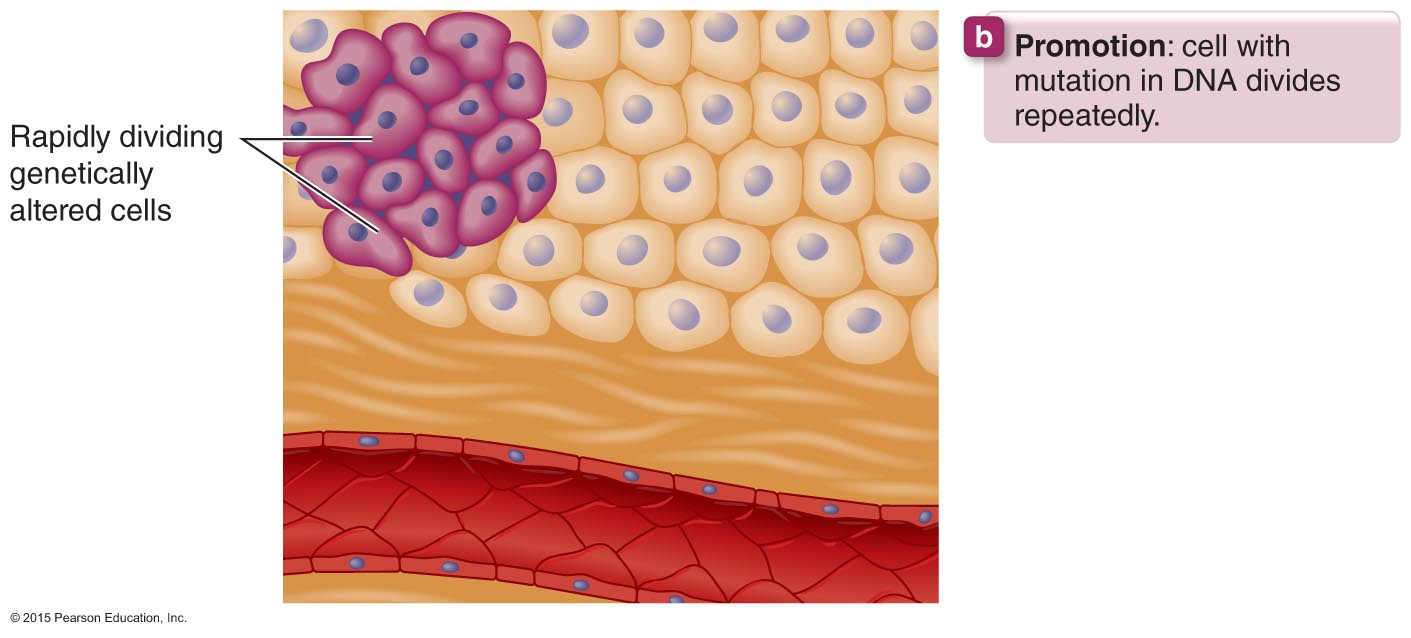
\includegraphics[width=\textwidth]{8_cancer_promotion}
	\caption{Cancer Promotion}
	\label{fig:cancer-promotion}
\end{figure}


\begin{figure}[H]
	\centering
	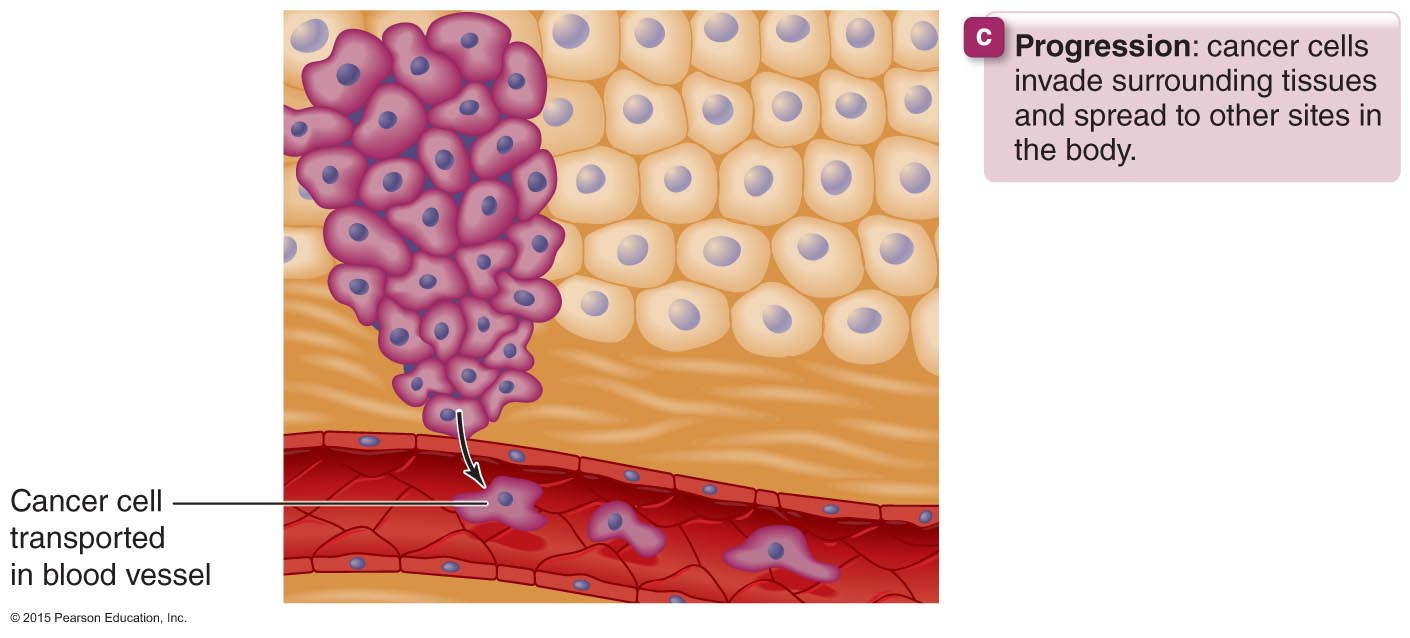
\includegraphics[width=\textwidth]{8_cancer_progression}
	\caption{Cancer Progression}
	\label{fig:cancer-progression}
\end{figure}

\begin{itemize}
	\item Factors that increase cancer risk include
	\begin{itemize}
		\item Family history of cancer
		\item Tobacco use
		\item Weight, poor diet, and sedentary lifestyle
		\item Infectious agents (e.g., STDs)
		\item Sun exposure (ultraviolet radiation)
	\end{itemize}
\end{itemize}

\begin{figure}[H]
	\centering
	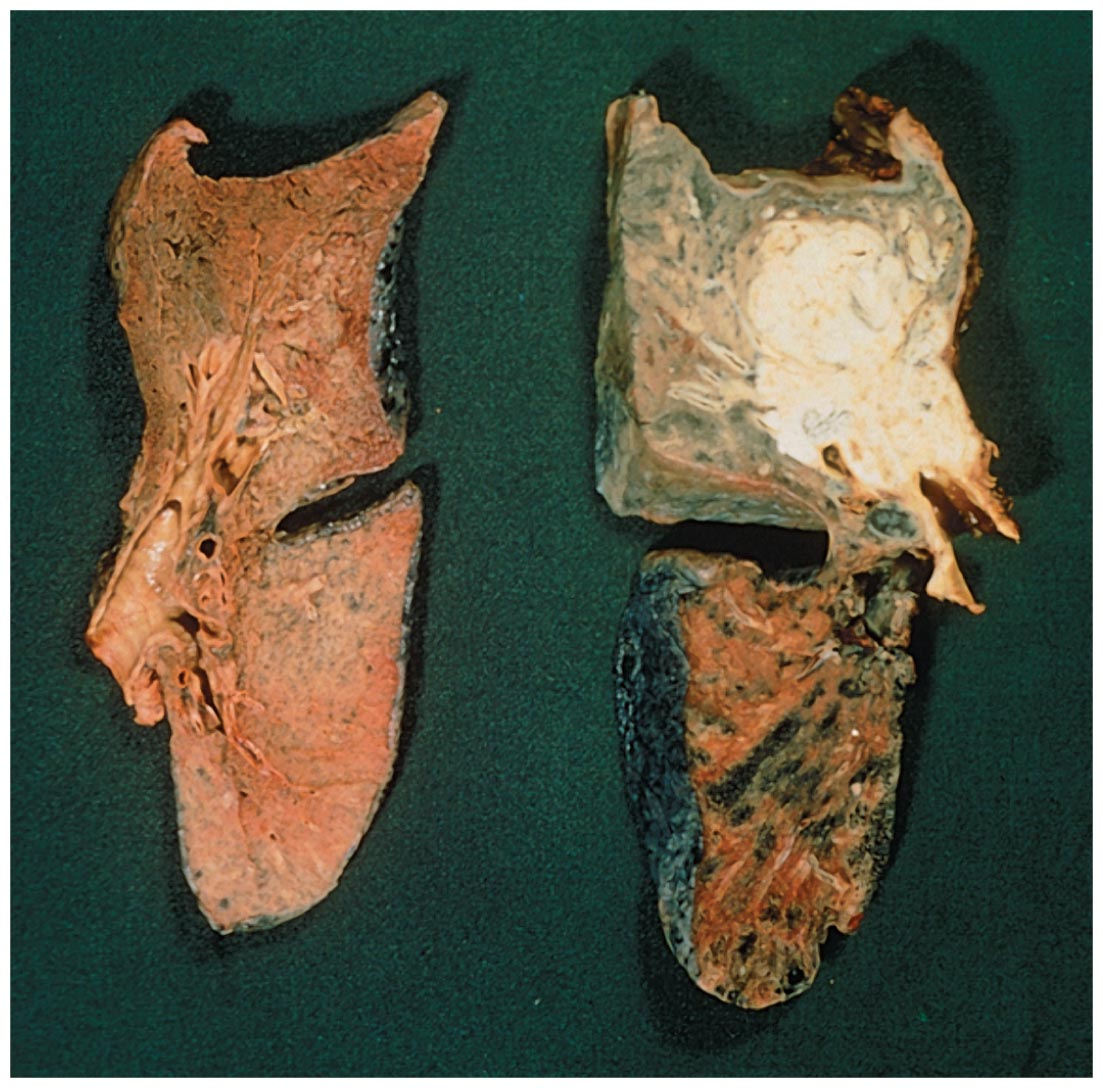
\includegraphics[width=\textwidth]{8_lungs}
	\caption{A Normal Lung and the Lung of a Smoker}
	\label{fig:lungs}
\end{figure}


\begin{figure}[H]
	\centering
	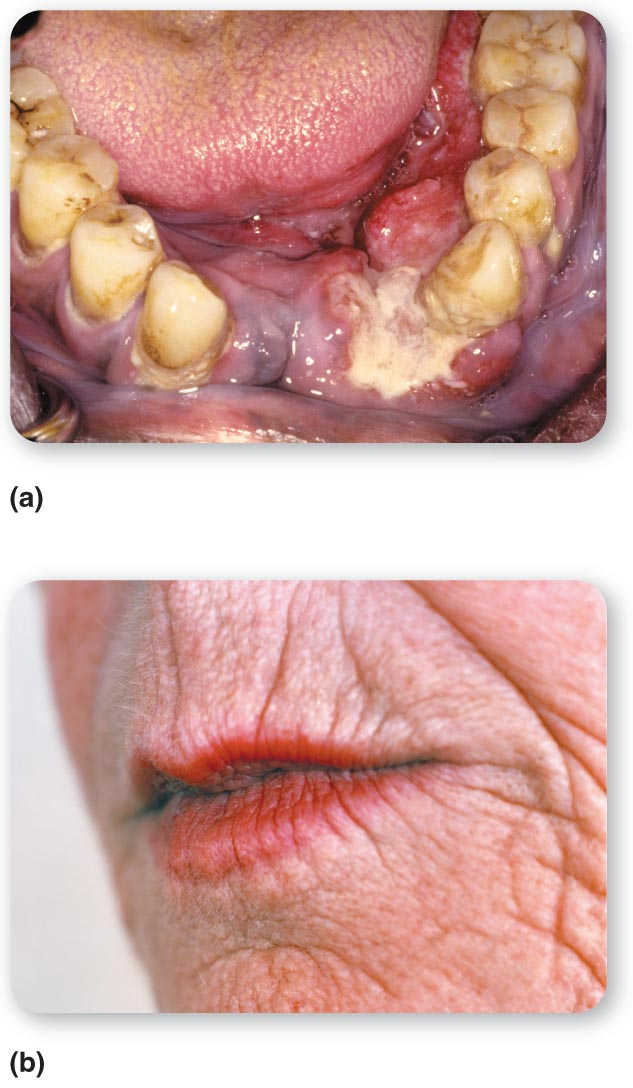
\includegraphics[height=0.75\paperheight]{8_tobacco_use_effects}
	\caption{Effects of Tobacco Use}
	\label{fig:tobacco-use-effects}
\end{figure}


\begin{figure}[H]
	\centering
	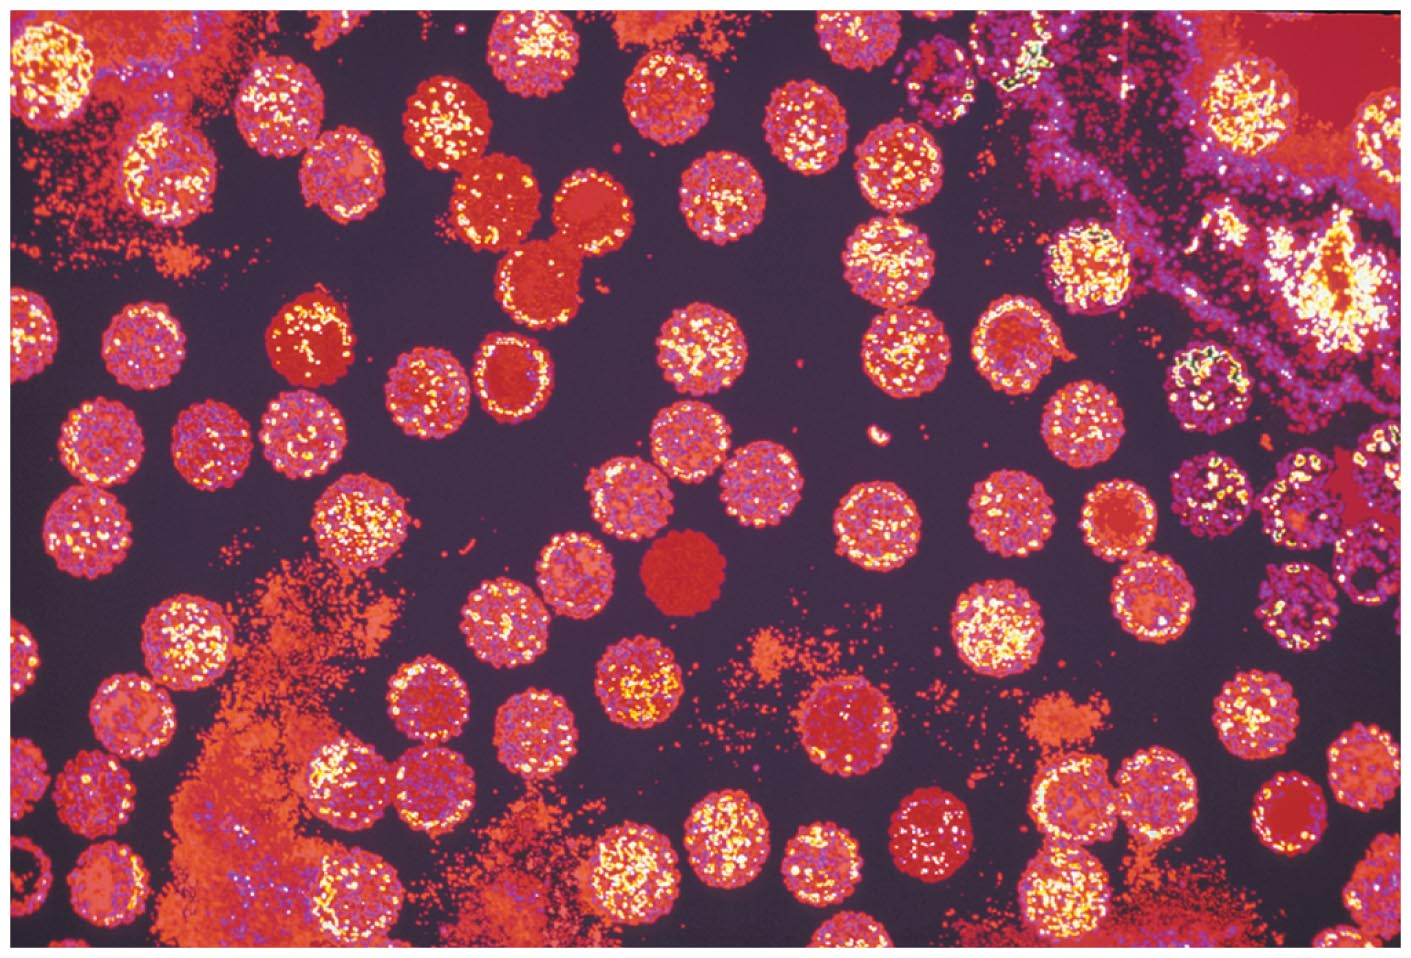
\includegraphics[width=\textwidth]{8_hpv}
	\caption{Human papillomavirus (HPV)}
	\label{fig:hpv}
\end{figure}


\begin{figure}[H]
	\centering
	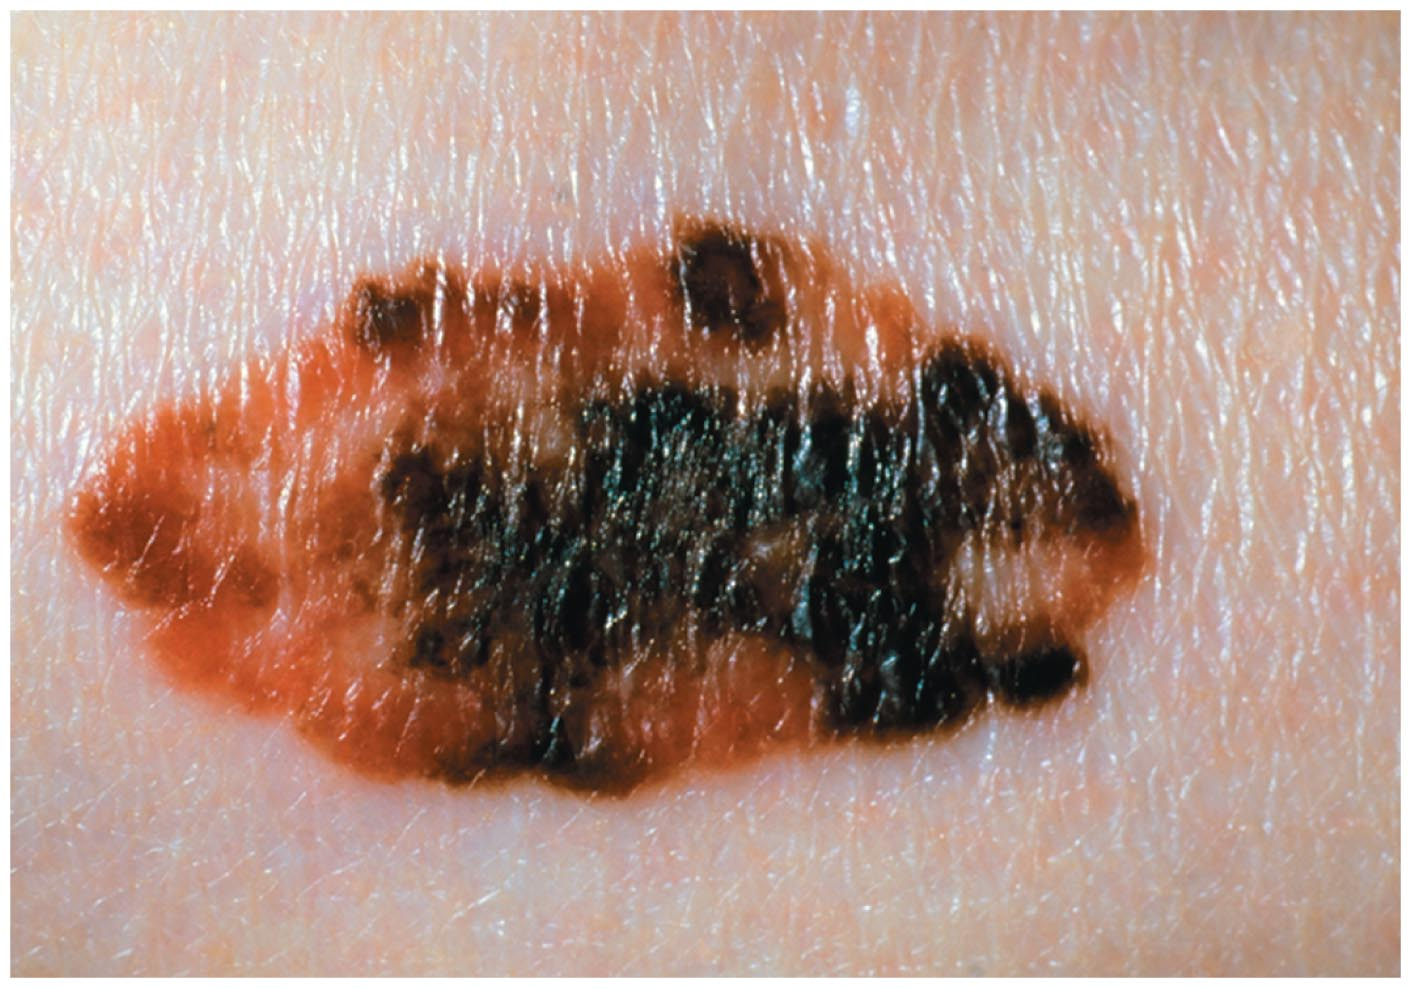
\includegraphics[width=\textwidth]{8_malignant_melanoma_lesion}
	\caption{A Lesion Associated with Malignant Melanoma}
	\label{fig:malignant_melanoma_lesion}
\end{figure}


\subsection{Signs and Symptoms of Cancer}\label{subsec:signs-and-symptoms-of-cancer}
\begin{itemize}
	\item Unexplained weight loss
	\item Fever
	\item Extreme fatigue
	\item Pain
	\item Skin changes
	\item Changes in bowel habits or bladder function
	\item Indigestion or trouble swallowing
	\item White patches inside the mouth or on the tongue
	\item Unusual bleeding or discharge
	\item Any thickening or lump
	\item Nagging cough or hoarseness
\end{itemize}

\subsection{Cancer Treatments}\label{subsec:cancer-treatments}
\begin{itemize}
	\item Treatment varies according to the location, the cell type, whether or not it has metastasized, and other individual factors
	\item Three major types of treatments:
	\begin{itemize}
		\item Surgery
		\item Radiation
		\item Chemotherapy
	\end{itemize}
\end{itemize}

\subsection{Cancer Prevention}\label{subsec:cancer-prevention}
\begin{description}
	\item[Check:] get screenings and exams
	\item[Quit:] stop smoking and alcohol abuse
	\item[Move:] get regular physical activity
	\item[Nourish:] maintain a recommended weight and eat a balanced, healthful diet
\end{description}

\subsection{Role of Antioxidants in Cancer}\label{subsec:Role of Antioxidants in Cancer}
\begin{itemize}
	\item Antioxidants may contribute to reducing the risk of cancer
	\item Antioxidants may reduce cancer risk by
	\begin{itemize}
		\item Enhancing the immune system
		\item Preventing oxidative damage to cells
		\item Inhibiting the growth of cancer cells and tumors
		\item Inhibiting the capacity of cancer cells to avoid aging and programmed cell death (apoptosis)
	\end{itemize}
\end{itemize}

\end{document}
